
%  template.tex for Biometrics papers
%
%  This file provides a template for Biometrics authors.  Use this
%  template as the starting point for creating your manuscript document.
%  See the file biomsample.tex for an example of a full-blown manuscript.



\documentclass[useAMS,referee]{biom}

\usepackage{amssymb}
\usepackage{booktabs}
\usepackage{multirow}
\usepackage{blkarray}
\usepackage{arydshln}
\usepackage{multirow}
\usepackage{mathtools}
\usepackage{amsmath,bm}
\usepackage{listings} 
\usepackage{blkarray}
\usepackage{footnote}
\usepackage{arydshln}
\usepackage{mathtools}
\usepackage{endrotfloat}
\usepackage{footnote}
\usepackage{natbib}
\usepackage[toc,page]{appendix}
\usepackage{graphicx}
\usepackage{tikz}
\usepackage{caption}
\usepackage[figurename=Figure,tablename=Table]{caption}
%\usepackage[tablename=Table]{caption}
\usetikzlibrary{matrix}
\usepackage{arydshln}
\usepackage{caption}


%  If your system does not have the AMS fonts version 2.0 installed, then
%  remove the useAMS option.
%
%  useAMS allows you to obtain upright Greek characters.
%  e.g. \umu, \upi etc.  See the section on "Upright Greek characters" in
%  this guide for further information.
%
%  If you are using AMS 2.0 fonts, bold math letters/symbols are available
%  at a larger range of sizes for NFSS release 1 and 2 (using \boldmath or
%  preferably \bmath).
% 
%  Other options are described in the user guide. Here are a few:
% 
%  -  If you use Patrick Daly's natbib  to cross-reference your 
%     bibliography entries, use the usenatbib option
%
%  -  If you use \includegraphics (graphicx package) for importing graphics
%     into your figures, use the usegraphicx option
% 
%  If you wish to typeset the paper in Times font (if you do not have the
%  PostScript Type 1 Computer Modern fonts you will need to do this to get
%  smoother fonts in a PDF file) then uncomment the next line
%  \usepackage{Times}

%%%%% PLACE YOUR OWN MACROS HERE %%%%%

\def\bSig\mathbf{\Sigma}
\newcommand{\VS}{V\&S}
\newcommand{\tr}{\mbox{tr}}

%  The rotating package allows you to have tables displayed in landscape
%  mode.  The rotating package is NOT included in this distribution, but
%  can be obtained from the CTAN archive.  USE OF LANDSCAPE TABLES IS
%  STRONGLY DISCOURAGED -- create landscape tables only as a last resort if
%  you see no other way to display the information.  If you do do this,
%  then you need the following command.

%\usepackage[figuresright]{rotating}

%%%%%%%%%%%%%%%%%%%%%%%%%%%%%%%%%%%%%%%%%%%%%%%%%%%%%%%%%%%%%%%%%%%%%

%  Here, place your title and author information.  Note that in 
%  use of the \author command, you create your own footnotes.  Follow
%  the examples below in creating your author and affiliation information.
%  Also consult a recent issue of the journal for examples of formatting.

\title[A bivariate framework to jointly model count and continuous responses]{A bivariate framework to jointly model count and continuous responses}

%  Here are examples of different configurations of author/affiliation
%  displays.  According to the Biometrics style, in some instances,
%  the convention is to have superscript *, **, etc footnotes to indicate 
%  which of multiple email addresses belong to which author.  In this case,
%  use the \email{ } command to produce the emails in the display.

%  In other cases, such as a single author or two authors from 
%  different institutions, there should be no footnoting.  Here, use
%  the \emailx{ } command instead. 

%  The examples below corrspond to almost every possible configuration
%  of authors and may be used as a guide.  For other configurations, consult
%  a recent issue of the the journal.

%  Single author -- USE \emailx{ } here so that no asterisk footnoting
%  for the email address will be produced.

%\author{John Author\emailx{email@address.edu} \\
%Department of Statistics, University of Warwick, Coventry CV4 7AL, U.K.}

%  Two authors from the same institution, with both emails -- use
%  \email{ } here to produce the asterisk footnoting for each email address

%\author{John Author$^{*}$\email{author@address.edu} and
%Kathy Authoress$^{**}$\email{email2@address.edu} \\
%Department of Statistics, University of Warwick, Coventry CV4 7AL, U.K.}

%  Exactly two authors from different institutions, with both emails  
%  USE \emailx{ } here so that no asterisk footnoting for the email address
%  is produced.

\author
{Maíra Blumer Fatoretto\emailx{mairafatoretto@gmail.com} \\
Department of Exact Sciences, University of São Paulo, Piracicaba, São Paulo, Brazil.
\and
Caroline Brophy\emailx{caroline.brophy@tcd.ie} \\
School of Computer Science and Statistics, Trinity College Dublin, Dublin 2, Ireland.
\and
Clarice Garcia Borges Demétrio\emailx{clarice.demetrio@usp.br} \\
Department of Exact Sciences, University of São Paulo, Piracicaba, São Paulo, Brazil.
\and
Rafael de Andrade Moral\emailx{rafael.deandrademoral@mu.ie} \\
Departament of Mathematics and Statistics, Maynooth University, Maynooth, Ireland.}

%  Three or more authors from same institution with all emails displayed
%  and footnoted using asterisks -- use \email{ } 

%\author{John Author$^*$\email{author@address.edu}, 
%Jane Author$^{**}$\email{jane@address.edu}, and 
%Dick Author$^{***}$\email{dick@address.edu} \\
%Department of Statistics, University of Warwick, Coventry CV4 7AL, U.K}

%  Three or more authors from same institution with one corresponding email
%  displayed

%\author{John Author$^*$\email{author@address.edu}, 
%Jane Author, and Dick Author \\
%Department of Statistics, University of Warwick, Coventry CV4 7AL, U.K}

%  Three or more authors, with at least two different institutions,
%  more than one email displayed 

%\author{John Author$^{1,*}$\email{author@address.edu}, 
%Kathy Author$^{2,**}$\email{anotherauthor@address.edu}, and 
%Wilma Flinstone$^{3,***}$\email{wilma@bedrock.edu} \\
%$^{1}$Department of Statistics, University of Warwick, Coventry CV4 7AL, U.K \\
%$^{2}$Department of Biostatistics, University of North Carolina at 
%Chapel Hill, Chapel Hill, North Carolina, U.S.A. \\
%$^{3}$Department of Geology, University of Bedrock, Bedrock, Kansas, U.S.A.}

%  Three or more authors with at least two different institutions and only
%  one email displayed

%\author{John Author$^{1,*}$\email{author@address.edu}, 
%Wilma Flinstone$^{2}$, and Barney Rubble$^{2}$ \\
%$^{1}$Department of Statistics, University of Warwick, Coventry CV4 7AL, U.K \\
%$^{2}$Department of Geology, University of Bedrock, Bedrock, Kansas, U.S.A.}


\begin{document}

%  This will produce the submission and review information that appears
%  right after the reference section.  Of course, it will be unknown when
%  you submit your paper, so you can either leave this out or put in 
%  sample dates (these will have no effect on the fate of your paper in the
%  review process!)

%\date{{\it Received October} 2007. {\it Revised February} 2008.  {\it
%Accepted March} 2008.}

%  These options will count the number of pages and provide volume
%  and date information in the upper left hand corner of the top of the 
%  first page as in published papers.  The \pagerange command will only
%  work if you place the command \label{firstpage} near the beginning
%  of the document and \label{lastpage} at the end of the document, as we
%  have done in this template.

%  Again, putting a volume number and date is for your own amusement and
%  has no bearing on what actually happens to your paper!  



%  This label and the label ``lastpage'' are used by the \pagerange
%  command above to give the page range for the article.  You may have 
%  to process the document twice to get this to match up with what you 
%  expect.  When using the referee option, this will not count the pages
%  with tables and figures.  

\label{firstpage}

%  put the summary for your paper here

\begin{abstract}
Multivariate data are present in many studies in the natural sciences. Generally, the interest is in more than one response variable and in how factors and covariates affect them, simultaneously. However, when the interest is in one count variable and one continuous variable, we need to use different approaches to model these variables jointly. In this work, motivated by a data set from entomology, in which a continuous and a count response were observed simultaneously, a novel mean-dispersion bivariate model was developed. The proposed model is based on the bivariate normal approximations, and adds a new parameter to the variance-covariance matrix to better accommodate the main characteristics of count data, such as overdispersion or underdispersion. This modelling framework showed good results and also allowed for greater flexibility in the case of heterogeneity of variances, and allows for the correlation between the two responses to vary according to an experimental treatment.
\end{abstract}

%  Please place your key words in alphabetical order, separated
%  by semicolons, with the first letter of the first word capitalized,
%  and a period at the end of the list.
%

\begin{keywords}
Count data; Entomology; Joint modelling; Multivariate data; Overdispersion; Poisson model; Underdispersion.
\end{keywords}

%  As usual, the \maketitle command creates the title and author/affiliations
%  display 

\maketitle

%  If you are using the referee option, a new page, numbered page 1, will
%  start after the summary and keywords.  The page numbers thus count the
%  number of pages of your manuscript in the preferred submission style.
%  Remember, ``Normally, regular papers exceeding 25 pages and Reader Reaction 
%  papers exceeding 12 pages in (the preferred style) will be returned to 
%  the authors without review. The page limit includes acknowledgements, 
%  references, and appendices, but not tables and figures. The page count does 
%  not include the title page and abstract. A maximum of six (6) tables or 
%  figures combined is often required.''

%  You may now place the substance of your manuscript here.  Please use
%  the \section, \subsection, etc commands as described in the user guide.

%

\section{Introduction}
\label{s:intro}

In many observational or experimental studies, multiple response variables are of interest, and they may be correlated. In statistical modelling techniques, multiple response variables can be analysed in isolation using univariate methods, where the dependence between them is not considered in the modelling. However, the correlation between the response variables can provide valuable insight, and their incorporation in the modelling framework can lead to more reliable tests and improved inference, especially when this correction is of high magnitude. Multivariate regression techniques facilitate the inclusion of correlated responses and are useful for exploring data patterns that may exist in more than one dimension ~\citep{raykov2008introduction,everitt2011introduction}. 

For the majority of univariate analysis, many inferential results are based on the normal distribution, and since many multivariate techniques are extensions of univariate analysis, the majority of multivariate procedures have the multivariate normal distribution as their underpinning. For example, in bivariate analysis, the relationship between two continuous variables with unbounded symmetric distribution could be described by a joint probability distribution using the bivariate normal density~\citep{jobson2012applied}. However, other distributions according to characteristics of the response variables can also be considered. The analysis of non-normal univariate or multivariate data involves, mostly, the generalized linear models (GLM) formulated by~\cite{nelder1972generalized}, that represent an elegant and encompassing mathematical framework to model response variables whose distribution belongs to the exponential family (such as normal, binomial, Poisson, gamma and inverse Gaussian). A feature of the exponential family of distributions is the  \textit{mean-variance} relationship, i.e., the fact that the variance is a function of the mean. 

~\cite{johnson1997multivariate} presented a range of discrete multivariate models that can jointly analyze count and binary data. Nevertheless, when it comes to joint modelling of one discrete and one continuous variable, suitable techniques and current software implementations are still emerging ~\citep{bonat2016multivariate}. Bonat et. al. (2018) proposed a flexible framework to model response variables of different nature jointly (e.g. unbounded and bounded continuous variables and discrete variables). They created the multivariate covariance generalized linear modelling framework (McGLM), implemented as the \texttt{mcglm} package for R software (R Core Team, 2022).~\nocite{team2022r} In their approach, marginal models are fitted through quasi-likelihood functions based on first and second-moment assumptions~\citep{bonat2017modelling,bonat2018multiple}. The framework includes flexibility in the specification of the covariance strucure and provides reliable tests for fixed effects. However, one drawback of this framework is that it does not provide an associated probability distribution. Another possibility for modelling discrete and continuous multivariate response variables jointly are copula models. The copula model allows us to incorporate the correlation between the variables and also allows flexibility when choosing the correlation structure, however, the use of different copulas generates completely different results~\citep{nikoloulopoulos2009modeling,krupskii2013factor}. In this paper, we present another option for modelling  count and continuous data jointly using an approximation based on the central limit theorem and an extension of the variance-covariance matrix. 

When analyzing count data, the Poisson model is a natural first choice, however, the Poisson distribution can be approximated asymptotically by the normal distribution~\citep{mood1950introduction}. A multivariate extension based on the normal distribution is advantageous in the sense that this distribution presents known and closed formulas.  A drawback of the Poisson model is the assumption of equality of mean and variance, which is not met very often in practice due to extra variability and other features, such as zero-inflation ~\cite{haslett2021modelling}. The overdispersion in count data may be caused by a deficiency of relevant covariates or heterogeneity of samples, or repeated measures, and it is necessary to model this extra variability to obtain reliable inference about the parameters ~\citep{hinde1998overdispersion,ver2007quasi}. Variance homogeneity is typically assumed for continuous data modelled by classical linear models based on the normal distribution; however, this variance assumption may not be reasonable or reflective of the real characteristics of the data. ~\cite{aitkin1987modelling} proposed the joint modelling of mean and dispersion in the normal regression analysis using a Fisher-scoring algorithm for the simultaneous maximum likelihood estimation. This proposal brought a powerful approach to deal with the heterogeneity of variance, which was modelled rather than being transformed away. ~\cite{mccullagh1989generalized} presented the joint modelling of mean and dispersion in the generalized linear models, using the extended quasi-likelihood function~\citep{nelder1987extended}. 





In this paper, we present a joint modelling of bivariate data, which also could be extended to multivariate data of more than two responses, to accommodate two counts, or two continuous response variables, or a combination of one count and one continuous variable using a bivariate normal distribution approximation. To obtain a versatile framework to deal with count and continuous data, we included an extra parameter in the variance-covariance matrix to capture different characteristics present in many situations. The normal bivariate model proposed allows us to model the mean and dispersion jointly, while dealing with over- and underdispersion, as well as variance heterogeneity. Furthermore, it is possible to fit the model considering different correlation structures that can change depending on a covariate of interest. To exemplify the method developed, we present a case study arising from the area of entomology.


This paper is organized as follows. Section 2 presents the case-study that is a motivation for this paper. Section 3 presents the bivariate framework to jointly model count and continuous responses. Section 4 presents estimation and inference for the novel regression model based on the maximum likelihood paradigm. The results from the analysis of the case study are presented in Section 5. The properties of the maximum likelihood and profile likelihood estimators are assessed in Section 6 through simulation studies. Finally, we present a discussion in Section 7.

% Assuming that there is this normal approximation for the count variables, we can incorporate new parameters in the variance-covariance matrix, modeling subdispersion and overdispersion even for multivariate data. 

% Therefore, the most fundamentals assumptions in multivariate analysis are normality,  homoscedasticity, independence of error, and linearity. Each of these issues should be addressed to some extent for each application of a multivariate technique ~\citep{hair1998multivariate}.


%Several models were proposed to model these errors, such as, the Mixed Models~\citep{carroll1988transformation,pinheiro2006mixed} and, the Generalized Linear Mixed Models for the GLM approach ~\citep{breslow1993approximate}. 




%introduced by Pregibon (1984)~\nocite{pregibon1984p}. In this approach the joint model is specified in terms of the dependence on covariates of the first two moments and the interlinking suggests an algorithm for the fit, once, the mean depends on the dispersion and the dispersion requires an estimate of the mean and, the estimated is assess






%In this paper, we present a new model for the analysis of bivariate data consisting of one count and one continuous variable, or both count or continuous variable, using a bivariate normal approximation. However this method coud also be extend to multivariate data. To obtain a versatility framework to deal with count data, we include a new parameters in the variance-covariance to capture different characteristics
%present in these distributions. 

%The double normal bivariate model proposed here is very flexible. First, it is possible to model jointly two responses, as in the classical bivariate model, and to considerer the correlation between them to estimate the others parameters present, even when there are different correlation, for example, by covariates. Thereby, the inferences could identify characteristics that were not possible in the univariate framework, for example, differences between treatments when the standard error taking account the correlation between the response variables. Also, this model include joint modelling of mean and dispersion, dealing with equal dispersion, overdispersion, underdispersion, and heteroscedastic errors, characteristics common in many structures of data, as count variables. 


\section{Case study - motivating example}


The data comes from an experiment examining \textit{Podisus nigrispinus} (Hemiptera: Pentatomidae), a predatory stinkbug found in agricultural and forest systems in several countries of Central and South America, when fed two different prey \textit{(Anticarsia gemmatalis} and \textit{Diatraea saccharalis}, two agricultural pests). 
This stinkbug has an important role as a biological control agent
for different crops, e.g., in forestry the predator can be useful to control defoliating caterpillars in \textit{Eucalyptus} plantations. The response variables are the weight and the fertility of female predators. The weight is one way of measuring the development of an insect over its life cycle, and the fertility measures how well the insect can establish itself in an ecosystem. 
Here, it is interesting to model these two variables together because an adequate diet can help to guarantee a high level of fertility. This information is essential for the choice of biological control strategies in pest management programmes~\citep{parra2002controle}. 

The experiment was carried out at the Laboratory of Forest Ecology and Entomology, Department of Entomology and Acarology, ESALQ - USP, Piracicaba, Brazil. The insects were placed in individualized incubator chambers, where they were fed and monitored daily. The two diets or treatments consisted of offering three caterpillars of either \textit{A. gemmatalis} or \textit{D. saccharalis} daily. The experiment started with 50 stinkbug insects for each diet, however, as there was a high mortality rate, the final measurements were made only with 9 replicates of the  \textit{A. gemmatalis} treatment and 18 of the \textit{D. saccharalis} treatment. After 18 days of receiving the diet, the weight of females was measured. Next, the females were allocated with a male that also received the same diet. The couples were kept until the death of the females. All eggs laid by the females were placed in Petri dishes and counted.

Looking at the scatter plot between female weight and number of eggs (see Figure \ref{fig1.1}), we see that stinkbugs being fed the \textit{A. gemmatalis} caterpillar diet performed more poorly overall than those fed the \textit{D. saccharalis} caterpillar diet. A strong correlation between female weight and number of eggs is observed for the \textit{D. saccharalis} diet; this indicates that a modelling approach that allows for varying correlation strength according to an experimental treatment could be suitable here.

\begin{figure}[htb]
	\centering
	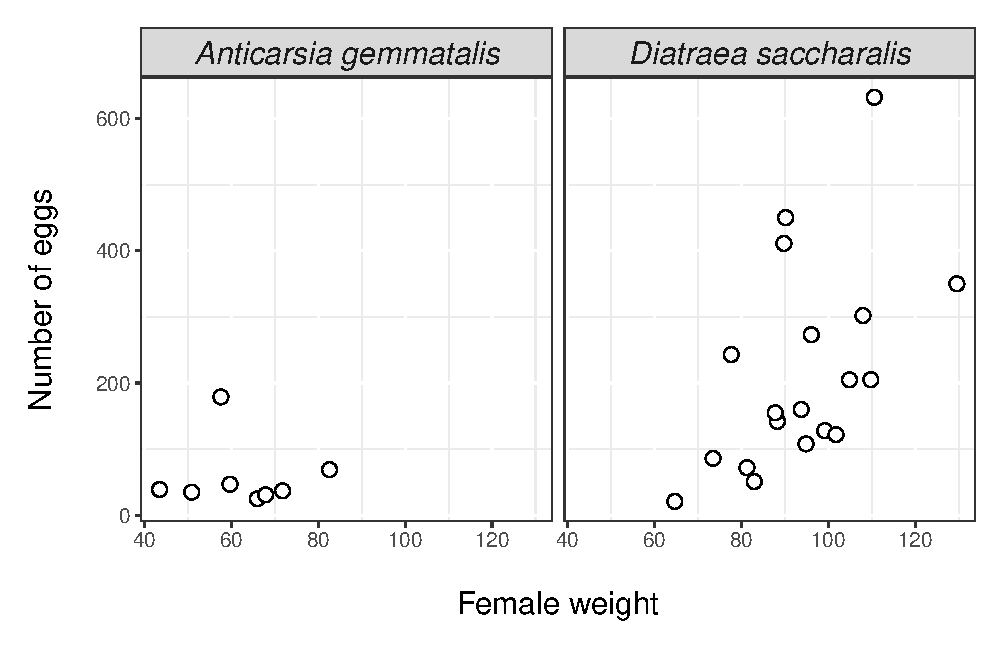
\includegraphics[width=0.8\textwidth]{pod1}
	\caption{\textit{Podisus nigrispinus} female weight after 18 days and total number of eggs laid throughout the insect's life cycle by treatment (diet consisting of \textit{Anticarsia gemmatalis} or \textit{Diatraea saccharalis}).}
	\label{fig1.1}
\end{figure}


\section{Joint Modelling of a Count and a Continuous Response}
\label{s:model}

%Bivariate models may be applied to analyse bivariate data jointly. However, when the outcomes have different distributions, the useful bivariate normal distribution may not capture all information present in the data. In this paper, we propose a joint modelling approach, based on the multivariate normal distribution, that is suitable for jointly analyzing count and continuous bivariate data. 

We propose the same marginal distribution structure for either a count or a continuous variable. Both assume a normal distribution, with mean $\boldsymbol{\mu_i}, i=1,2$ and standard deviation $\boldsymbol{\phi_i}\boldsymbol{\mu_i}, i=1,2$, which depends on the mean and a dispersion parameter $\phi_i$. It is also possible to capture variance heterogeneity, overdispersion, or underdispersion by incorporating covariates in the dispersion parameters. We model the mean $\boldsymbol{\mu}$ through a monotonic and differentiable link function $\boldsymbol{\mathbf{g}(\mu) = \eta}$, such that the linear predictor is $\boldsymbol{\eta} = \mathbf{X}\boldsymbol{\beta}$, with $\mathbf{X}$ a design matrix and $\boldsymbol{\beta}$ a vector of regression parameters.

Let $\mathbf{Y_1}$ and $\mathbf{Y_2}$ be vectors of count or continuous random variables. We then assume that, marginally, $\mathbf{Y_1} \sim N(\boldsymbol{\mu_1},\boldsymbol{\Sigma_1})$ and  $\mathbf{Y_2} \sim N(\boldsymbol{\mu_2},\boldsymbol{\Sigma_2})$, with the joint distribution of $\mathbf{Y_1}$ and $\mathbf{Y_2}$ taken to be multivariate normal, i.e.,

\begin{align}\label{eq1}
\begin{bmatrix}\mathbf{Y_1}\\
\mathbf{Y_2}
\end{bmatrix} &\sim  N
\begin{pmatrix}
\begin{bmatrix}
\boldsymbol{\mu_1}\\
\boldsymbol{\mu_2}
\end{bmatrix}\!\!,&
\begin{bmatrix}
\boldsymbol{\Sigma_1} & \boldsymbol{\Sigma_{12}} \\
\boldsymbol{\Sigma_{12}} & \boldsymbol{\Sigma_2}
\end{bmatrix}
\end{pmatrix},
\end{align}
where  $\boldsymbol{\Sigma_1}$ denotes the variance-covariance matrix for the first response; $\boldsymbol{\Sigma_2}$ denotes the variance-covariance matrix for the second response and $\boldsymbol{\Sigma_{12}}$
denotes the covariance matrix between the two responses, where $\boldsymbol{\Sigma_{12}}$ depends on a correlation parameter $\rho$, $\boldsymbol{\Sigma_1}$ and $\boldsymbol{\Sigma_2}$.

We write  $$\boldsymbol{\Sigma_i} = \mathbf{D_\phi}\mathbf{D_\mu},$$ where $\mathbf{D_\phi}=\mbox{diag}(\mathbf{X}_\phi \boldsymbol{\phi})$, $\mathbf{D_\beta}=\mbox{diag} (g^{-1}(\mathbf{X}_\beta \boldsymbol{\beta}))$, and the function $\mbox{diag}(\mathbf{x})$ is defined as a square matrix with the elements of the vector $\mathbf{x}$ in its main diagonal; $\mathbf{X_\phi}$ and $\mathbf{X_\beta}$ are the design  matrices for the dispersion and mean parameters respectively; and $\boldsymbol\phi$ and $\boldsymbol\beta$ unknown parameter vectors. This yields
\begin{center}
	$\boldsymbol{\Sigma_i} =
	\begin{pmatrix}
	\phi_{i1}\mu_{i1} & 0 & \dots & 0 \\
	0 & \phi_{i2}\mu_{i2} & \dots & 0 \\
	\vdots & \vdots & \ddots & \vdots \\
	0 & 0 & \dots & \phi_{in}\mu_{in}
	\end{pmatrix}
	$,
\end{center}
where $i\in\{1,2\}$ is the index corresponding to each response variable and $j=1,\ldots,n$ is the index corresponding to each observation.


\section{Estimation and Inference}

We first show how estimation works for a single response, and in the next subsection extend it to the bivariate case of interest here. 

\subsection{Univariate modelling}\label{univariate}

Taking one of the response outcomes $\mathbf {Y} _i $, from here we will omit the index $ i $ to improve readability. We assume that asymptotically  $\boldsymbol{Y} \sim N({\boldsymbol{\mu}},\boldsymbol{\Sigma}= \mathbf{D_\phi}\mathbf{D_\mu})$, and write the log-likelihood as
\begin{equation}\label{eq22}
\begin{array}{l}
\log \mathcal{L}(\boldsymbol{\mu},\boldsymbol{\Sigma}| \mathbf{y})= l(\boldsymbol{\mu},\boldsymbol{\Sigma}| \mathbf{y})= -\frac{1}{2}\{\log |\boldsymbol{\Sigma}| +  (\mathbf{y}-\boldsymbol{\mu})'\boldsymbol{\Sigma}^{-1} (\mathbf{y}-\boldsymbol{\mu})\} + \mbox{constant}



%= -\frac{1}{2}\log |\mathbf{D_\phi}\mathbf{D_\mu}| - \frac{1}{2} (\mathbf{y}-\boldsymbol{\mu})'(\mathbf{D_\phi}\mathbf{D_\mu})^{-1} (\mathbf{y}-\boldsymbol{\mu})\\~\\

%  =	\{- \frac{1}{2}\log|\mathbf{D_\phi}|-  \frac{1}{2} \log|\mathbf{D_\mu}|  - \frac{1}{2} (\mathbf{y}-\boldsymbol{\mu})'(\mathbf{D_\phi}\mathbf{D_\mu})^{-1} (\mathbf{y}-\boldsymbol{\mu}) \}

\end{array}
\end{equation}

The estimating equations can be obtained using the chain rule. Differentiating (\ref{eq22}) w.r.t. $\boldsymbol{\Sigma}$ yields 

\begin{equation}\label{eq4}
\begin{array}{l}
\dfrac{\partial l}{\partial \boldsymbol{\Sigma}} = -\frac{1}{2}(\boldsymbol{\Sigma}^{-1})'+\frac{1}{2}(\boldsymbol{\Sigma}^{-1})'+(\mathbf{y}-\boldsymbol{\mu})(\mathbf{y}-\boldsymbol{\mu})'(\boldsymbol{\Sigma}^{-1})'+.

\end{array}
\end{equation}

Now further differentiating eq. (\ref{eq4}) w.r.t. $\mathbf{D_\phi}$ and  w.r.t. $\boldsymbol{\phi}$ yields
\begin{equation}\label{eq5}
\begin{array}{l}
-\frac{1}{2}\mbox{diag}\mathbf{ (X_\phi \boldsymbol{\phi})^{-1}}\circ \mathbb{I}+\frac{1}{2}\mbox{diag}\mathbf{ (X_\phi \boldsymbol{\phi})^{-1}D_\mu^{-1}}(\mathbf{y}-\boldsymbol{\mu})(\mathbf{y}-\boldsymbol{\mu})'\mbox{diag}\mathbf{( X_\phi \boldsymbol{\phi})^{-1}}\circ \mathbb{I},
\end{array}
\end{equation}
where $\mathbb{I}$ is an $n \times n$ identity matrix and $\mathbb{J}$ is an $n \times 1$ vector of 1s, and $\circ$ the Hadamard product. Finally, solving eq. (\ref{eq5}) w.r.t. $\boldsymbol{\phi}$ yields
\begin{equation}\label{eq6}
\boldsymbol{\hat{\phi}} = \mathbf{(X_\phi'X_\phi)^{-1}X_\phi'}\mathbf{\{(D_\mu^{-1}}(\mathbf{y}-\boldsymbol{\mu})(\mathbf{y}-\boldsymbol{\mu})'\circ \mathbb{I}) \mathbb{J}\},
\end{equation}
see Appendix A for details on calculations. In this case, for positive values, the dispersion parameter ($\phi$) is always greater than zero, with $\phi < 1$ resulting in underdispersion and $\phi>1$ in overdispersion.

It is not as straightforward to obtain the maximum likelihood estimator for $\boldsymbol{\beta}$, because $\boldsymbol{\mu}$ is also a function of $\boldsymbol{\Sigma}$ in the likelihood. Therefore we employ an iterative procedure, using estimates of the regression coefficients using the known estimator for the regression parameters in linear models as starting values, and then updating $\hat{\boldsymbol{\beta}}$ using $\boldsymbol{\hat{\mu}}$ estimated in the preceding stage. The maximum likelihood estimator (MLE) of $\boldsymbol{\beta}$, conditional on $\boldsymbol{\mu},\boldsymbol{\phi},\boldsymbol{\rho}$ is given by ~\citep{laird1982random,molenberghs2000linear}
\begin{center}
$\boldsymbol{\hat{\beta}(\mu},\boldsymbol{\phi},\boldsymbol{\rho}) =  \mathbf{(X'\boldsymbol{\Sigma}}^{-1}\mathbf{X)^{-1} X'\boldsymbol{\Sigma}}^{-1}\mathbf{Y}$.
\end{center} 


Because we are including different link functions,  not limited to the identity, we include a matrix of weights $\mathbf{W}$ in the estimation of $\boldsymbol{\beta}$, following the estimation procedure of the GLM framework. The estimation for the vector $\boldsymbol{\beta}$ is given considering
\begin{equation}
\boldsymbol{\eta} = \mathbf{g}(\mathbf{\mu})\textnormal{,}  \qquad \mathbf{W} = \dfrac{\textnormal{1}}{\boldsymbol{\Sigma}[\mathbf{g}'(\boldsymbol{\mu})]^2} \quad \mbox{and} \quad \boldmath{\textbf{z} = \eta + \mathbf{G}(\textbf{y} - \mu)}\textnormal{,}
\end{equation}  
where $\textbf{W}$ is a diagonal matrix of weights, $\boldsymbol{\Sigma} = \mathbf{D_\phi D_\mu}$ and $\textbf{G} =$diag$\{g'(\mu_1),\dots,g'(\mu_n)\}$ ~\citep{nelder1972generalized,mccullagh1989generalized}.

Using $\boldsymbol{\eta^{(1)}} = \mathbf{g}(\mathbf{y})$ for the first iteration, then



\begin{equation}\label{estimatorregression}
\hat{\boldsymbol{\beta}}^{(1)}= \mathbf{(X'X)^{-1} X'\boldsymbol{\eta}}^{(1)}\qquad \mbox{and} \qquad \hat{\boldsymbol{\beta}}^{(n)} = \mathbf{(X'W}^{(n-1)}\mathbf{X)^{-1} X'W}^{(n-1)}\textbf{z}^{(n-1)}.
\end{equation}

This algorithm yields the same results as numerically maximising the likelihood function using, e.g. the BFGS algorithm, however it is much faster in terms of computational burden. We will show that these estimators are unbiased in the simulation studies in Section 6.

%Para $m=2, \dots , k$, sendo $k-1$ o número necessário de iterações para convergência, pode ser resumido as estimativas:\\
%(1) Obter as estimativas\\

%\begin{center}
%	$\boldsymbol{\eta}^{m} = \mathbf{X}\boldsymbol{\beta}^{(m)}$ and $\boldsymbol{\mu}^{(m)} = \exp \{\mathbf{X}\boldsymbol{\beta}^{(m)}\}$
%\end{center}

%(2) Obter a variável dependente ajustada:
%\begin{center}
%$\mathbf{z^{(m)}} = \log(\boldsymbol{\mu}^{(m)})+ \dfrac{(\mathbf{y} - \boldsymbol{\mu}^{(m)})}{\boldsymbol{\mu}^{(m)}}$
%\end{center}
%e os pesos

%\begin{center}
%	$\mathbf{w^{(m)}} = \dfrac{\boldsymbol{\phi}}{\boldsymbol{\mu^{(m)}}}$
%\end{center}
%and 
%(3) calcular

%\begin{center}
%	$	\boldsymbol{\beta}^{(m+1)} = (\mathbf{X^{T}W^{(m)}X)^{-1} X^ {T}W^{(m)}z^{(m)}}$
%\end{center}


\subsection{Bivariate modelling}

To model both outcomes jointly it is necessary to estimate the covariance matrix $\boldsymbol{\Sigma}_{12}$ (eq. \ref{eq1}). Martinez and Benedito (2013)~\nocite{martinez2013general}introduced a method to construct the multivariate covariance matrix using Kronecker products. Bonat and J{\o}rgersen (2016) applied the same method to develop the technique called Multivariate Covariance Generalized Linear Models.
Let $\mathbf{Y}_{n(2 \times 1)} = \{\mathbf{Y}_1,\mathbf{Y}_2\} $, where the response variables are stacked, with $n = \mbox{number of observations}$ and $2 = \mbox{number of outcomes}$; $\boldsymbol{\Sigma}_i$ the $n \times n$ covariance matrix within the outcome $i$ for $i = 1,2$. Let $\boldsymbol{\Sigma}_b$ be the $R \times R$ correlation matrix between outcomes, with the diagonal elements equal to $1$ and off-diagonal elements equal to $\rho$. 
Then 
\begin{equation*}
\mbox{E}(\mathbf{Y})	 = \{g^{-1}(\mathbf{X}_1 \boldsymbol{\beta}_1), g^{-1}(\mathbf{X}_2 \boldsymbol{\beta}_2)\} 
\end{equation*}
\begin{equation}\label{variance}	
\mbox{Var}(\mathbf{Y})=\boldsymbol{\Sigma}= \mbox{Bdiag}(\tilde{\boldsymbol{\Sigma}}_1, \tilde{\boldsymbol{\Sigma}}_2)(\boldsymbol{\Sigma}_b \otimes \mathbf{I} )\mbox{Bdiag}(\tilde{\boldsymbol{\Sigma}}_1',  \boldsymbol{\tilde{\Sigma}}_2')
\end{equation}
where the matrix $\boldsymbol{\tilde{\Sigma}}_i$ denotes the lower triangular matrix of the Cholesky decomposition of $\boldsymbol{\Sigma}_i$. The operator Bdiag denotes a block diagonal matrix and $\mathbf{I}$ denotes an $n \times n$ identity matrix. Then, the covariance matrix, presented in the (eq. \ref{eq1})., will be defined as 

%Then, the covariance matrix, could be defined as
\begin{center}
$\boldsymbol{\Sigma}_{12} = \rho  \tilde{\boldsymbol{\Sigma}}_{1} \tilde{\boldsymbol{\Sigma}}_{2}^{T} $.
\end{center}
Here we propose an extension to allow more than one correlation coefficient, for example, we could have one for each treatment in our case study data (Section 2). This requires increasing the flexibility of the $(\boldsymbol{\Sigma}_b\otimes \mathbf{I})$ matrix to include more than one correlation coefficient.   
Let $\mathbf{X}_\rho$ denote a $N \times t$ design matrix, with $t$ the number of treatment levels, and $\boldsymbol{\rho}$ a vector for the correlation coefficients  with $t \times 1$ dimension, then writing $\boldsymbol{\Sigma}_\rho=	\mbox{diag}(\mathbf{X}_\rho \boldsymbol{\rho})$ and replacing $(\boldsymbol{\Sigma}_b\otimes \mathbf{I})$ in eq. (\ref{variance}), we have
\begin{equation*}	
\mbox{Var}(\mathbf{Y})=\boldsymbol{\Sigma}= \mbox{Bdiag}(\tilde{\boldsymbol{\Sigma}}_1, \tilde{\boldsymbol{\Sigma}}_2)
\left[\begin{array}{cc}
\mathbf{I} & \boldsymbol{\Sigma}_\rho\\
\boldsymbol{\Sigma}_\rho & \mathbf{I} \end{array} \right]
\mbox{Bdiag}(\tilde{\boldsymbol{\Sigma}}_1', \boldsymbol{\tilde{\Sigma}}_2').
\end{equation*}

For $\mathbf{Y} = \mathbf{[Y_1,Y_2]}$, the full log likelihood is
\begin{equation}\label{16}
l(\boldsymbol{\mu},\boldsymbol{\Sigma(\mu,\phi,\rho)}| \mathbf{y}) = -\frac{1}{2}\{\log |\boldsymbol{\Sigma}| +  (\mathbf{y}-\boldsymbol{\mu})'\boldsymbol{\Sigma}^{-1} (\mathbf{y}-\boldsymbol{\mu})\} + \mbox{constant}.
\end{equation}
The covariance matrix is more flexible, allowing the modelling of data sets that have subgroups with different correlation profiles. A likelihood ratio test can be used to test if correlations coefficients differ, for example by levels of a treatment in an experiment. 

J{\o}rgensen and Knudsen (2004)~\nocite{jorgensen2004parameter}suggested a method to jointly estimate all parameters of the $\boldsymbol{\Sigma}$ matrix using the Newton scoring algorithm, based on quasi-likelihood and the Pearson estimating functions, applying second-moment assumptions. As an estimation alternative approach, here, the matrices $\boldsymbol{\Sigma_1}$ and $\boldsymbol{\Sigma_2}$ are estimated first separately, using the maximum likelihood method, presented in section (\ref{univariate}). These estimates are then used as initial values to obtain the estimates $\boldsymbol{\hat\rho}$ by profiling the log-likelihood function w.r.t. $\boldsymbol{\rho}$ and maximizing (\ref{16}) numerically. At each step, the estimates for $\boldsymbol{\mu}$ and $\boldsymbol{\phi}$ are updated, using the estimation algorithm described in Section 4.1. Since the derivatives of $l$ w.r.t. $\boldsymbol{\rho}$ cannot be obtained in closed form, the  \texttt{L-BFGS-B} algorithm~\citep{zhu1997algorithm} was used. Standard errors for the regression parameters are obtained based on the observed information matrix $\mathbf{I}(\boldsymbol\theta)$, where $\textbf{I}\boldsymbol(\theta)= - \textbf{H}\boldsymbol(\theta)$ (hessian matrix) is calculated by numerical approximation of $l(\boldsymbol\theta)$, using Richardson extrapolation, as implemented in the \texttt{hessian()} function of the \texttt{numDeriv} package~\citep{gilbert2006numderiv}. Since $\hat{\boldsymbol{\phi}}$ depends on $\hat{\boldsymbol{\beta}}$, the standard errors for the dispersion parameters are obtained using a two-stage algorithm. First, considering $\boldsymbol{\hat\rho}$, we obtain the standard errors for $\boldsymbol{\hat\beta}$ . In the next stage considering $\boldsymbol{\hat\rho}$ and $\boldsymbol{\hat\beta}$ we obtain the standard errors for $\boldsymbol{\hat\phi}$.

We applied these methods to the case study data described in Section 2. Diagnostic analyses and goodness-of-fit assessment for the models fitted to the case study data set were carried out by producing bivariate residual plots with simulation polygons~\citep{moral2020bivariate}. Likelihood-ratio tests were used to compare treatments and to assess the significance of the estimated effects.



\section{Case study analysis}


We fitted the bivariate model to the data set described in Section 2, with the log and identity link functions for the count and continuous outcome respectively, including the effects of diet (treatment) in the linear predictors for the mean, dispersion and correlation. Table \ref{table0} shows the estimated parameters and standard errors. The females fed with \textit{D. saccharalis} emerged with greater weight ($\hat\beta_{22}$) and had greater fertility, producing more eggs $(\hat\beta_{12}$). The estimates $\hat\phi_{11}$ and $\hat\phi_{12}$ indicate overdispersion for the number of eggs,  however since their standard errors are large we tested for their equality. The estimates $\hat\phi_{21}$ and $\hat\phi_{22}$ are also similar.

\begin{table}[htb]
\caption{Parameter estimates and standard errors (S.E.) for
the normal bivariate model. $\beta_{11}$ and $\beta_{12}$ represent the mean number of eggs produced by stinkbugs on for diets \textit{Anticarsia gemmatalis} and \textit{Diatraea saccharalis} respectively; $\beta_{21}$ and $\beta_{22}$ represent the mean weight for stinkbugs on diets \textit{A. gemmatalis} and \textit{D. saccharalis} respectively. $\phi_{11}$ and $\phi_{12}$ represent the dispersion of the number of eggs for diets \textit{A. gemmatalis} and \textit{D. saccharalis} respectively; $\phi_{21}$ and $\phi_{22}$ represent the dispersion of weight for diets \textit{A. gemmatalis} and \textit{D. saccharalis} respectively. $\rho_1$ represents the correlation between number of eggs and weight for \textit{A. gemmatalis} diet and the parameter $\rho_2$ represents the correlation between number of eggs and weight for \textit{D. saccharalis}.}
\label{table0}
\begin{center}
\begin{tabular}{lrr}
	\hline
	Parameter & Estimate & S.E. \\ \hline
	$\beta_{11}$ & 4.0561 & 0.2907 \\ 
	$\beta_{12}$ &  5.3782 & 0.1609 \\
	
	$\beta_{21}$& 62.5000 & 4.0684  \\
	
	$\beta_{22}$& 93.9474 & 3.3824\\
	
	$\phi_{11}$& 39.0292 & 19.5049 \\ 
	$\phi_{12}$&  106.6240  & 32.1814\\
	$\phi_{21}$&  2.1186 & 1.0588  \\ 
	$\phi_{22}$& 2.3138 &0.6983\\
	$\rho_1$ & -0.0389 & 0.3528 \\
	
	$\rho_2$& 0.5192 & 0.1487\\
	\hline
	\multicolumn{2}{l}{Log-Likelihood} & -221.0125 \\
	\hline
\end{tabular}
\end{center}
\end{table}


The bivariate residual plot with simulation polygons with 99 simulations showed 3 out of 27 points out of their respective polygons, which indicates a reasonably good fit (Figure \ref{fig1.2}). 




\begin{figure}[htb]
\centering
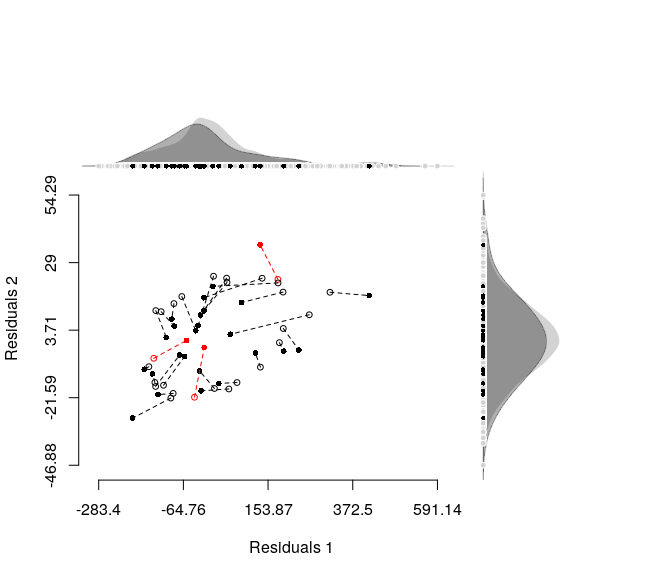
\includegraphics[width=0.7\textwidth]{pod4}
\caption{Bivariate plot with simulation polygons assuming a bivariate normal distribution for raw bivariate residuals, with estimated marginal densities at the top and right-hand side of the plot. The lighter shade corresponds to the estimated density of all simulated diagnostics, and the darker one corresponds to the estimated density of the observed diagnostics. The points outside their simulated polygons are displayed in red.}
\label{fig1.2}
\end{figure}



The selection of the model was performed using likelihood-ratio tests. We assessed the treatment effect on the mean and the dispersion by each outcome and jointly (Table \ref{table2} and \ref{table5.3}). The effect of treatment on the correlation was also tested and presented no significance, but here due to the differences in correlations observed per treatment (Figure \ref{fig1.1}), the biological assumption, and the small sample size, we chose to maintain a different correlation effect per treatment.  The \textit{D. saccharallis} presented an estimated value for the correlation of 0.5192 indicating that the insects that received this diet produced more eggs as they gained more weight, contributing to their development, but for the
\textit{A. gemmatalis} diet we did not see this same relationship, since the estimated value for the correlation was -0.0389.

Considering the dispersion parameters, the test gave evidence for equal dispersion coefficients, but different regression coefficients for each diet. The regression parameters showed a difference between treatments for both outcomes, hence, the diet \textit{D. saccharalis} contributed to a better development of the predator.

%The estimates also showed high overdispersion for the number of eggs and heterogeneity of variance for the female weight, and a small correlation between outcomes.

\begin{table}[htb]
\centering
\caption{Model fit measurements and comparisons between the complete and reduced models to test the treatment effect on the mean and on the dispersion for each outcome.}
\begin{tabular}{p{6cm}p{1cm}crr} \hline
Model & np & \textit{l} & 2(diff \textit{l}) & $P(> \chi^2)$ \\ 		\hline
Full model & 10 & -221.0125 && \\
\hdashline
\qquad	$\beta_{11} = \beta_{12}$   & 9 &$-227.4322$ & 12.8394& 0.0003\\
\qquad	$\beta_{21} = \beta_{22}$   & 9 &$-236.2779$ & 16.4631& $<0.0001$\\

\qquad $\phi_{10} = \phi_{11}$  & 9 & $-222.2381$ & 2.4511& 0.2936\\

\qquad  $\phi_{20} = \phi_{21}$  & 9 &$-221.0235$ & 0.02209& 0.9890\\


\hline
\end{tabular}

\footnote{}{np, number of parameters; \textit{l}, log-likelihood; diff \textit{l}, difference in log-likelihoods.}	

\label{table2}
\end{table}


\begin{table}[htb]
\centering
\caption{Model fit measurements and comparisons between the complete and reduced models to test the treatment effect on the mean and on the dispersion for both outcomes jointly.}
\begin{tabular}{p{6cm}p{1cm}crr} \hline
Model & np & \textit{l} & 2(diff \textit{l}) & $P(> \chi^2)$ \\ 		\hline
Full model & 10 & -221.0125 && \\
\hdashline
\qquad	$\beta_{11} = \beta_{12}$ and $\beta_{21} = \beta_{22}$   & 8 &$-232.1660$ & 22.3070& $<0.0001$\\

\qquad $\phi_{10} = \phi_{11}$ and $\phi_{20} = \phi_{21}$   & 8 & $-222.2347$ & 2.4445& 0.2946\\


\hline
\end{tabular}

\footnote{}{np, number of parameters; \textit{l}, log-likelihood; diff \textit{l}, difference in log-likelihoods.}	

\label{table5.3}
\end{table}


%\begin{table}[!h]
%	\centering
%	\caption{Parameter estimates (EST.) and standard errors (SE) for
%		the normal bivariate model. $\beta_{11}$ and $\beta_{12}$ represent the mean of number of eggs for diets \textit{Anticarsia} and \textit{Diatraea} respectively; $\beta_{21}$ and $\beta_{22}$ represent the mean of weight for for diets \textit{Anticarsia} and \textit{Diatraea} respectively. $\phi_{1}$  represents the dispersion mean of number of eggs for diets \textit{Anticarsia} and \textit{Diatraea}; $\phi_{2}$ represents the dispersion mean of weight for diets \textit{Anticarsia} and \textit{Diatraea}, and  $\rho$ represents the correlation between number of eggs and weight.}
%	\begin{tabular}{lrr}\Hline
%		&EST. & SE \\ 		\hline
%		$\beta_{11}$ & 4.0561 &  0.3744\\ 
%		$\beta_{12}$ &  5.3782 & 0.1430\\
%		
%		$\beta_{21}$& 62.5000 & 4.0810  \\
%		
%		$\beta_{22}$& 93.9474 & 3.3274  \\
%		$\phi_{1}$& 86.5959 & 22.5908 \\ 
%		$\phi_{2}$&  2.2560 & 0.5885  \\ 
%		$\rho$ & 0.4031  & 0.1495 \\
%		\hline
%		LogLik & -222.8309
%		& \\
%		\hline

%	\end{tabular}
%	\label{table3}
%\end{table}



\section{Simulation studies}\label{Simulation}

Simulation studies were performed to assess the properties of the maximum likelihood estimators and the flexibility of the bivariate framework. The scenarios proposed here compare the performance of the proposed model with different sample size; under, over and equidispersion for the count outcome; heterogeneity of variances for the continuous outcome and negative, positive, low and high correlation between outcomes.

We conducted the simulation studies based on the experimental structure described in our case study (Section 2). Four scenarios were designed considering one treatment factor with two levels and the numbers of experimental units equal to with half of the experiments units assigned to each treatment. The count outcome was generated from a normal distribution with a logarithmic link function, fixing the regression coefficients at the values $\beta_{11}=2$ and $\beta_{12}=3$ (the first index represents the response variable and the second index the treatment level). The dispersion parameters were fixed at the values $\phi_{11}=0.5$ and $\phi_{12}=2$. For the second continuous outcome, we considered $\beta_{21}=10$, $\beta_{22}=300$, $\phi_{21}=1$, $\phi_{22}=10$ and an identity link function. We produced simulations based on four different values for a single correlation parameter ($\rho = -0.8, 0.2, 0.5$ and $0.8$). These scenarios present negative, weak, moderate, and strong positive correlation. To check the consistency of the estimators, four sample sizes were considered: 50, 100, 300, and 600. We generated 1000 data sets for each scenario. The simulation process is summarised as follows
\begin{enumerate}
\item Define	$\boldsymbol{\beta_1}$=$\begin{bmatrix}\mathbf{2}\\
\mathbf{3}
\end{bmatrix}$; $\boldsymbol{\beta_2}$=$\begin{bmatrix}\mathbf{10}\\
\mathbf{300}
\end{bmatrix}$;	
$\boldsymbol{\phi_1}$=$\begin{bmatrix}\mathbf{0.5}\\
\mathbf{2}
\end{bmatrix}$;	
$\boldsymbol{\phi_2}$=$\begin{bmatrix}\mathbf{1}\\
\mathbf{10}
\end{bmatrix}$;\\

\item Set up $\mathbf{X}_{\beta_1}$ and  $\mathbf{X}_{\beta_2}$  as  $n \times 2$ design matrices;

\item Set up  $\mathbf{X}_{\phi_1}$ and $\mathbf{X}_{\phi_2}$ as  $n \times 2$ dispersion design matrices;


\item Calculate $\boldsymbol{\mu_1} = g^{-1}(\mathbf{X}_{\beta_1}\boldsymbol{\beta_1}) = \exp(\mathbf{X}_{\beta_1}\boldsymbol{\beta_1})$ and 
$\boldsymbol{\mu_2} = g^{-1}(\mathbf{X}_{\beta_2}\boldsymbol{\beta_2}) = \mathbf{X}_{\beta_2}\boldsymbol{\beta_2}$;

\item Obtain $\boldsymbol{\Sigma_1} = \mbox{diag}(\mathbf{X}_{\phi_1} \boldsymbol{\phi_1}) \mbox{diag} (\boldsymbol{\mu_1}) $ and	
$\boldsymbol{\Sigma_2} = \mbox{diag}(\mathbf{X}_{\phi_2} \boldsymbol{\phi_2}) \mbox{diag} (\boldsymbol{\mu_2}) $;

\item Set up  $\mathbf{X}_{\rho}$ as an $n \times 1$ unit matrix; 

\item Obtain $\boldsymbol{\Sigma}_\rho=	\mbox{diag}(\mathbf{X}_\rho{\rho})$, where $\rho$ is a scalar
($-0.8$, 0.2, 0.5 or 0.8);\\

\item Calculate $	\boldsymbol{\Sigma}= \mbox{Bdiag}({\boldsymbol{\Sigma}}_1, {\boldsymbol{\Sigma}}_2)
\left[\begin{array}{cc}
\mathbf{I} & \boldsymbol{\Sigma}_\rho\\
\boldsymbol{\Sigma}_\rho & \mathbf{I} \end{array} \right]
\mbox{Bdiag}({\boldsymbol{\Sigma}}_1^{T}, \boldsymbol{{\Sigma}}_2^{T})$;\\


\item Simulate from $	\begin{bmatrix}\mathbf{Y_1}\\
\mathbf{Y_2}
\end{bmatrix} \sim  N
\begin{pmatrix}
\begin{bmatrix}
\boldsymbol{\mu_1}\\
\boldsymbol{\mu_2}
\end{bmatrix}\!\!,&
\boldsymbol{\Sigma}
\end{pmatrix}
$;\\

\item Fit the proposed model to the simulated data sets and evaluate estimates.

\end{enumerate}

This process was followed for each simulation scenario.
Further, we also simulated a scenario with two correlations parameters, one for each treatment. The study considered 1,000 simulations, sample sizes equal to 50, 100 and 300, and four scenarios combining correlation coefficients ($\rho_1=0.2$ and $\rho_2=0.5$; $\rho_1=0.2$ and $\rho_2=0.8$; $\rho_1=-0.8$ and $\rho_2=0.2$; $\rho_1=-0.2$ and $\rho_2=0.5$).

The complete code used for the simulations and model fitting can be found in the supplementary materials.





\subsection{Simulation results}

% In this section, we present the results of the simulation studies described above.

To visualize estimation bias for each simulation scenario Figure \ref{fig1.3}
was constructed. It presents the average bias, defined as the average estimate of 1,000 simulations minus the true value and their respective confidence interval calculated as the average bias plus and minus 1.96 times the standard error.

\begin{figure}[htb]
\centering
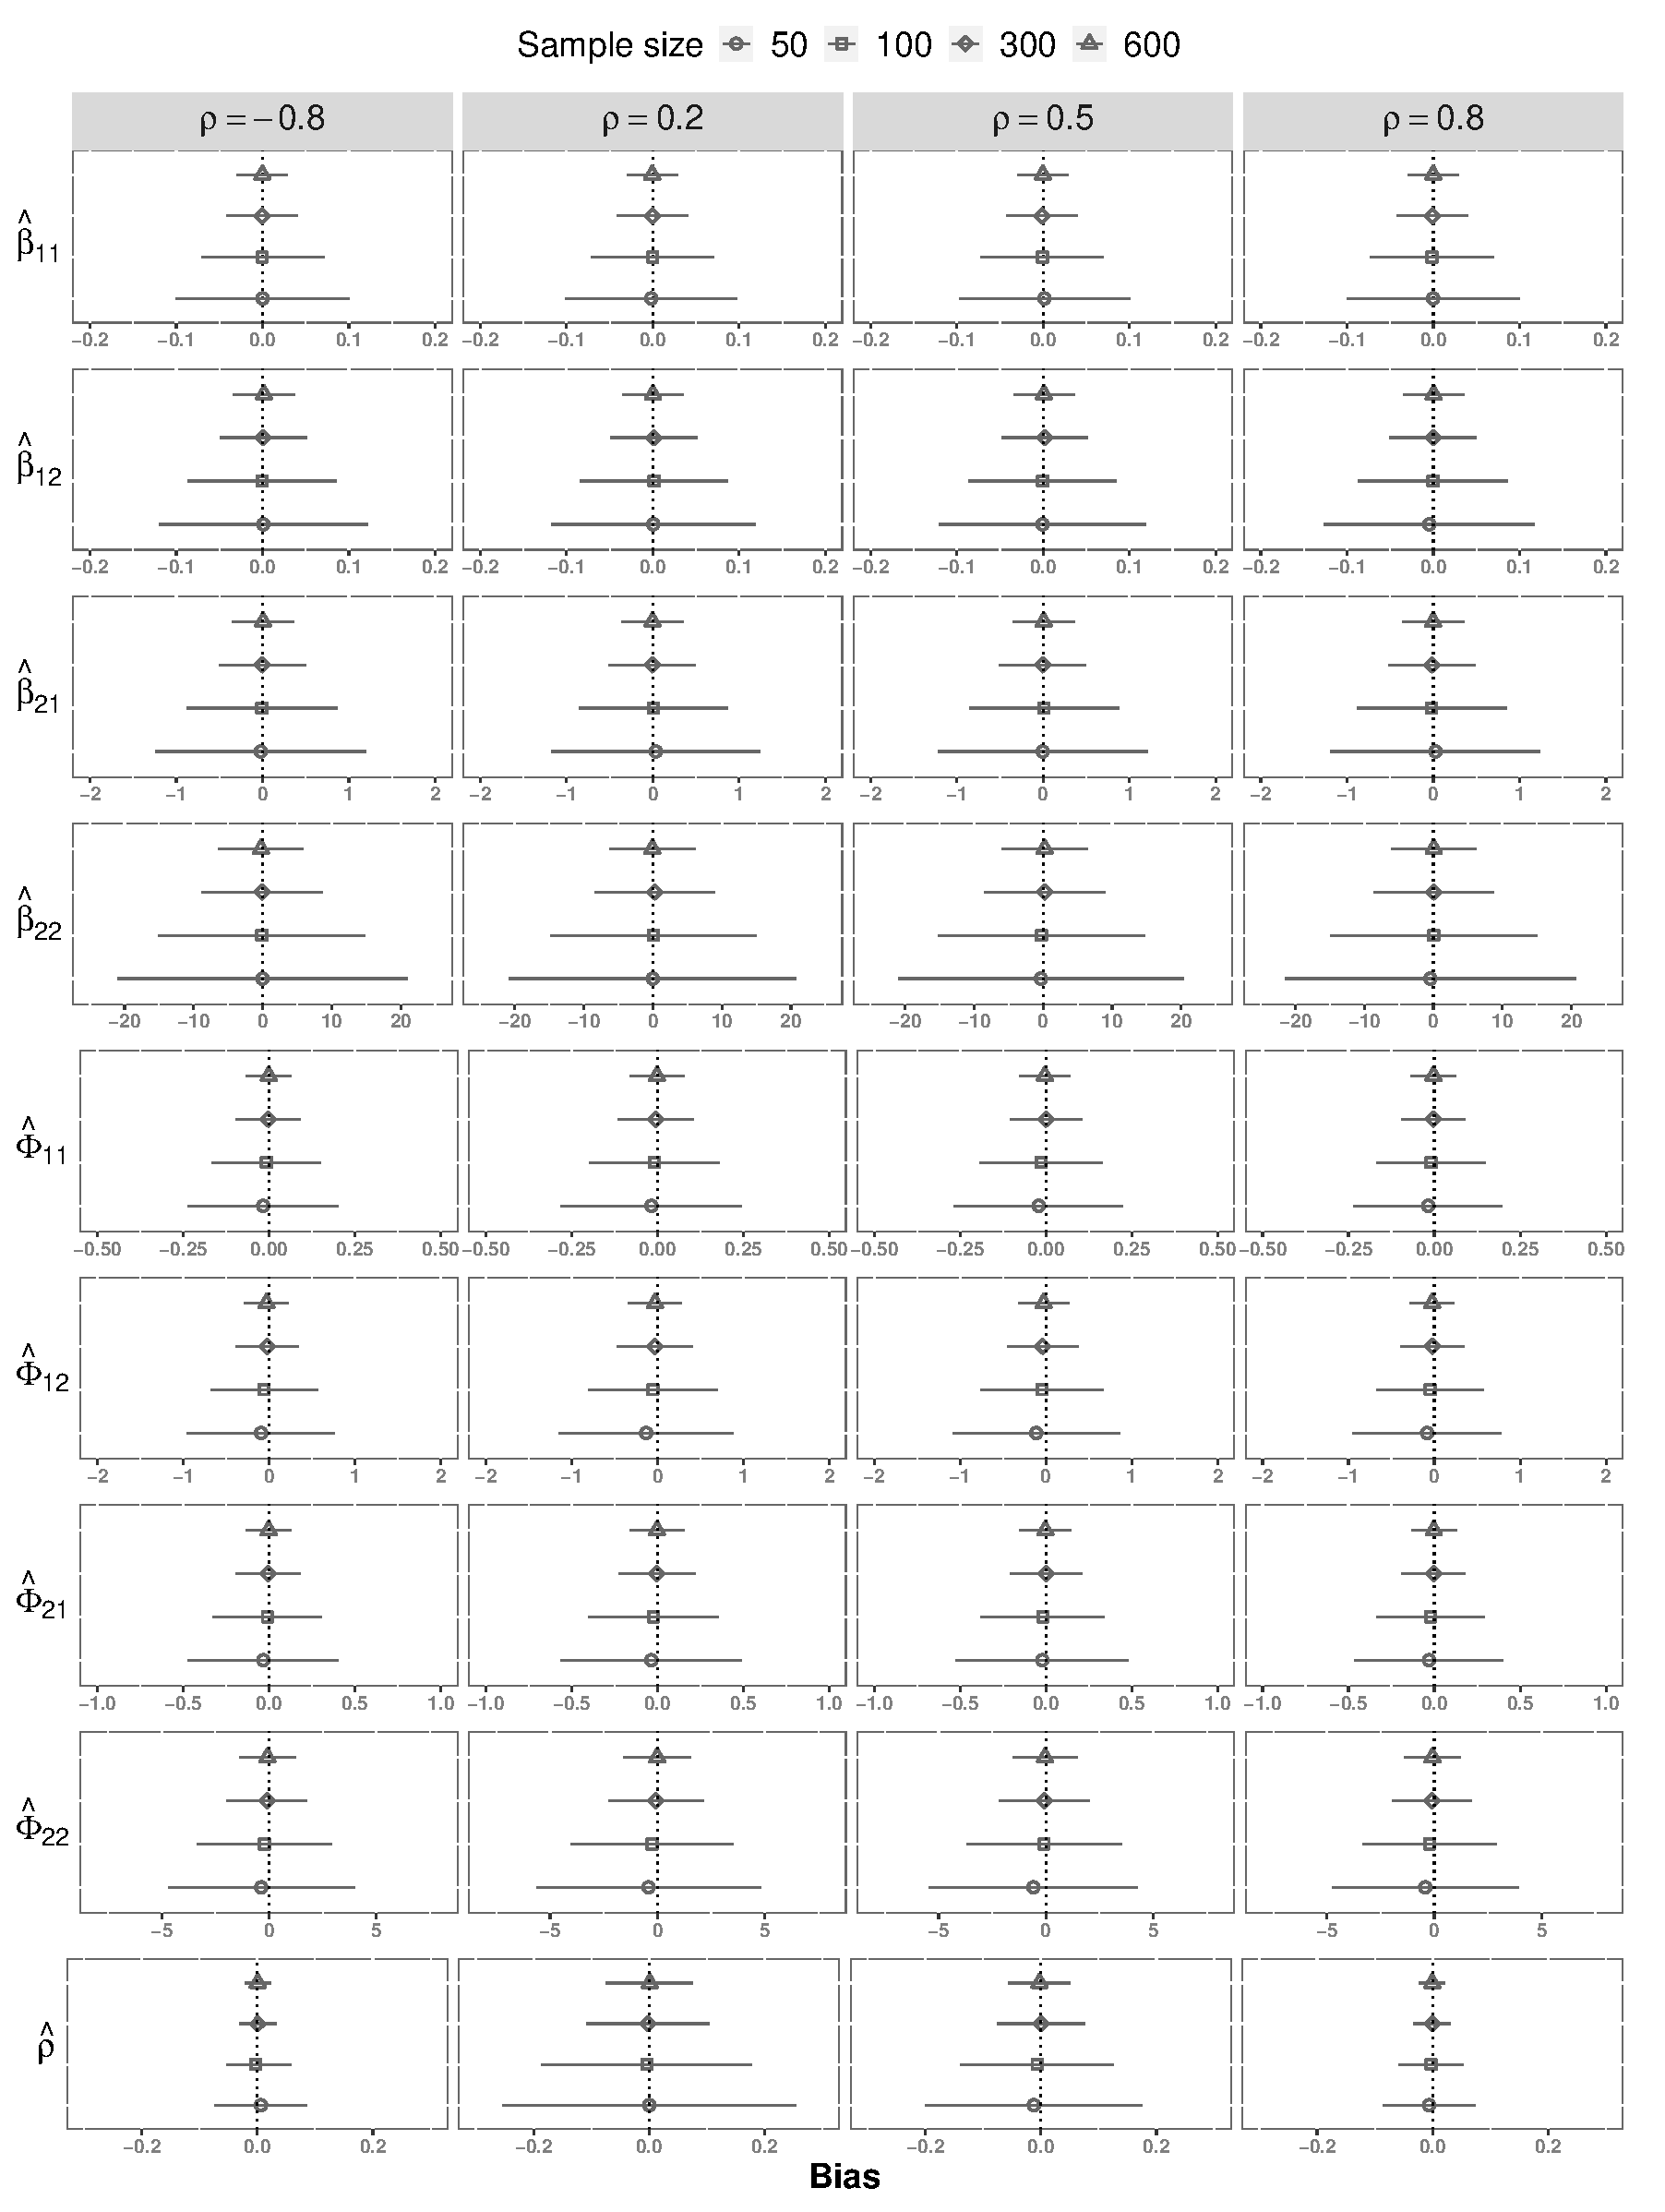
\includegraphics[width=.98\textwidth]{Figure_2}
\caption{Estimation average bias of each simulation scenario (symbols) with their respective 95\% confidence intervals, considering 1,000 simulations.}
\label{fig1.3}
\end{figure}

The results of the simulation studies showed that for all correlation levels, the average bias and the standard errors tend to zero as the sample size increases, meaning that all parameters have unbiased and consistent estimators. This is also observed for the regression parameters when the correlation is very high ($\rho = 0.8$). For the correlation parameters, the bias is low even for small samples, but it is smaller when the sample size increases. The average standard error is lower for strong correlations, positive or negative ($\rho = -0.8$ and $\rho = 0.8$); this is clear for the correlation coefficient, but it is also possible to observe a slightly smaller average standard error for the dispersion coefficients.

Figure \ref{fig1.4} shows the empirical coverage rate of the asymptotic confidence intervals. The results showed that for the regression parameters the empirical coverage rates are close to the nominal level of $95\%$ for all sample sizes and all simulation scenarios. For the dispersion and correlation parameters, the empirical coverage rates are lower than the nominal level, however, for $\rho = 0.2$ and $\rho = 0.5$, they become closer to the nominal level for large samples. The worst scenario is with a small sample and strong correlation, in this case, even for large samples the coverage rate is still lower than the nominal level. An alternative here is to consider other methods to construct the confidence intervals such as the bootstrap approach. 


\begin{figure}[htb]
\centering
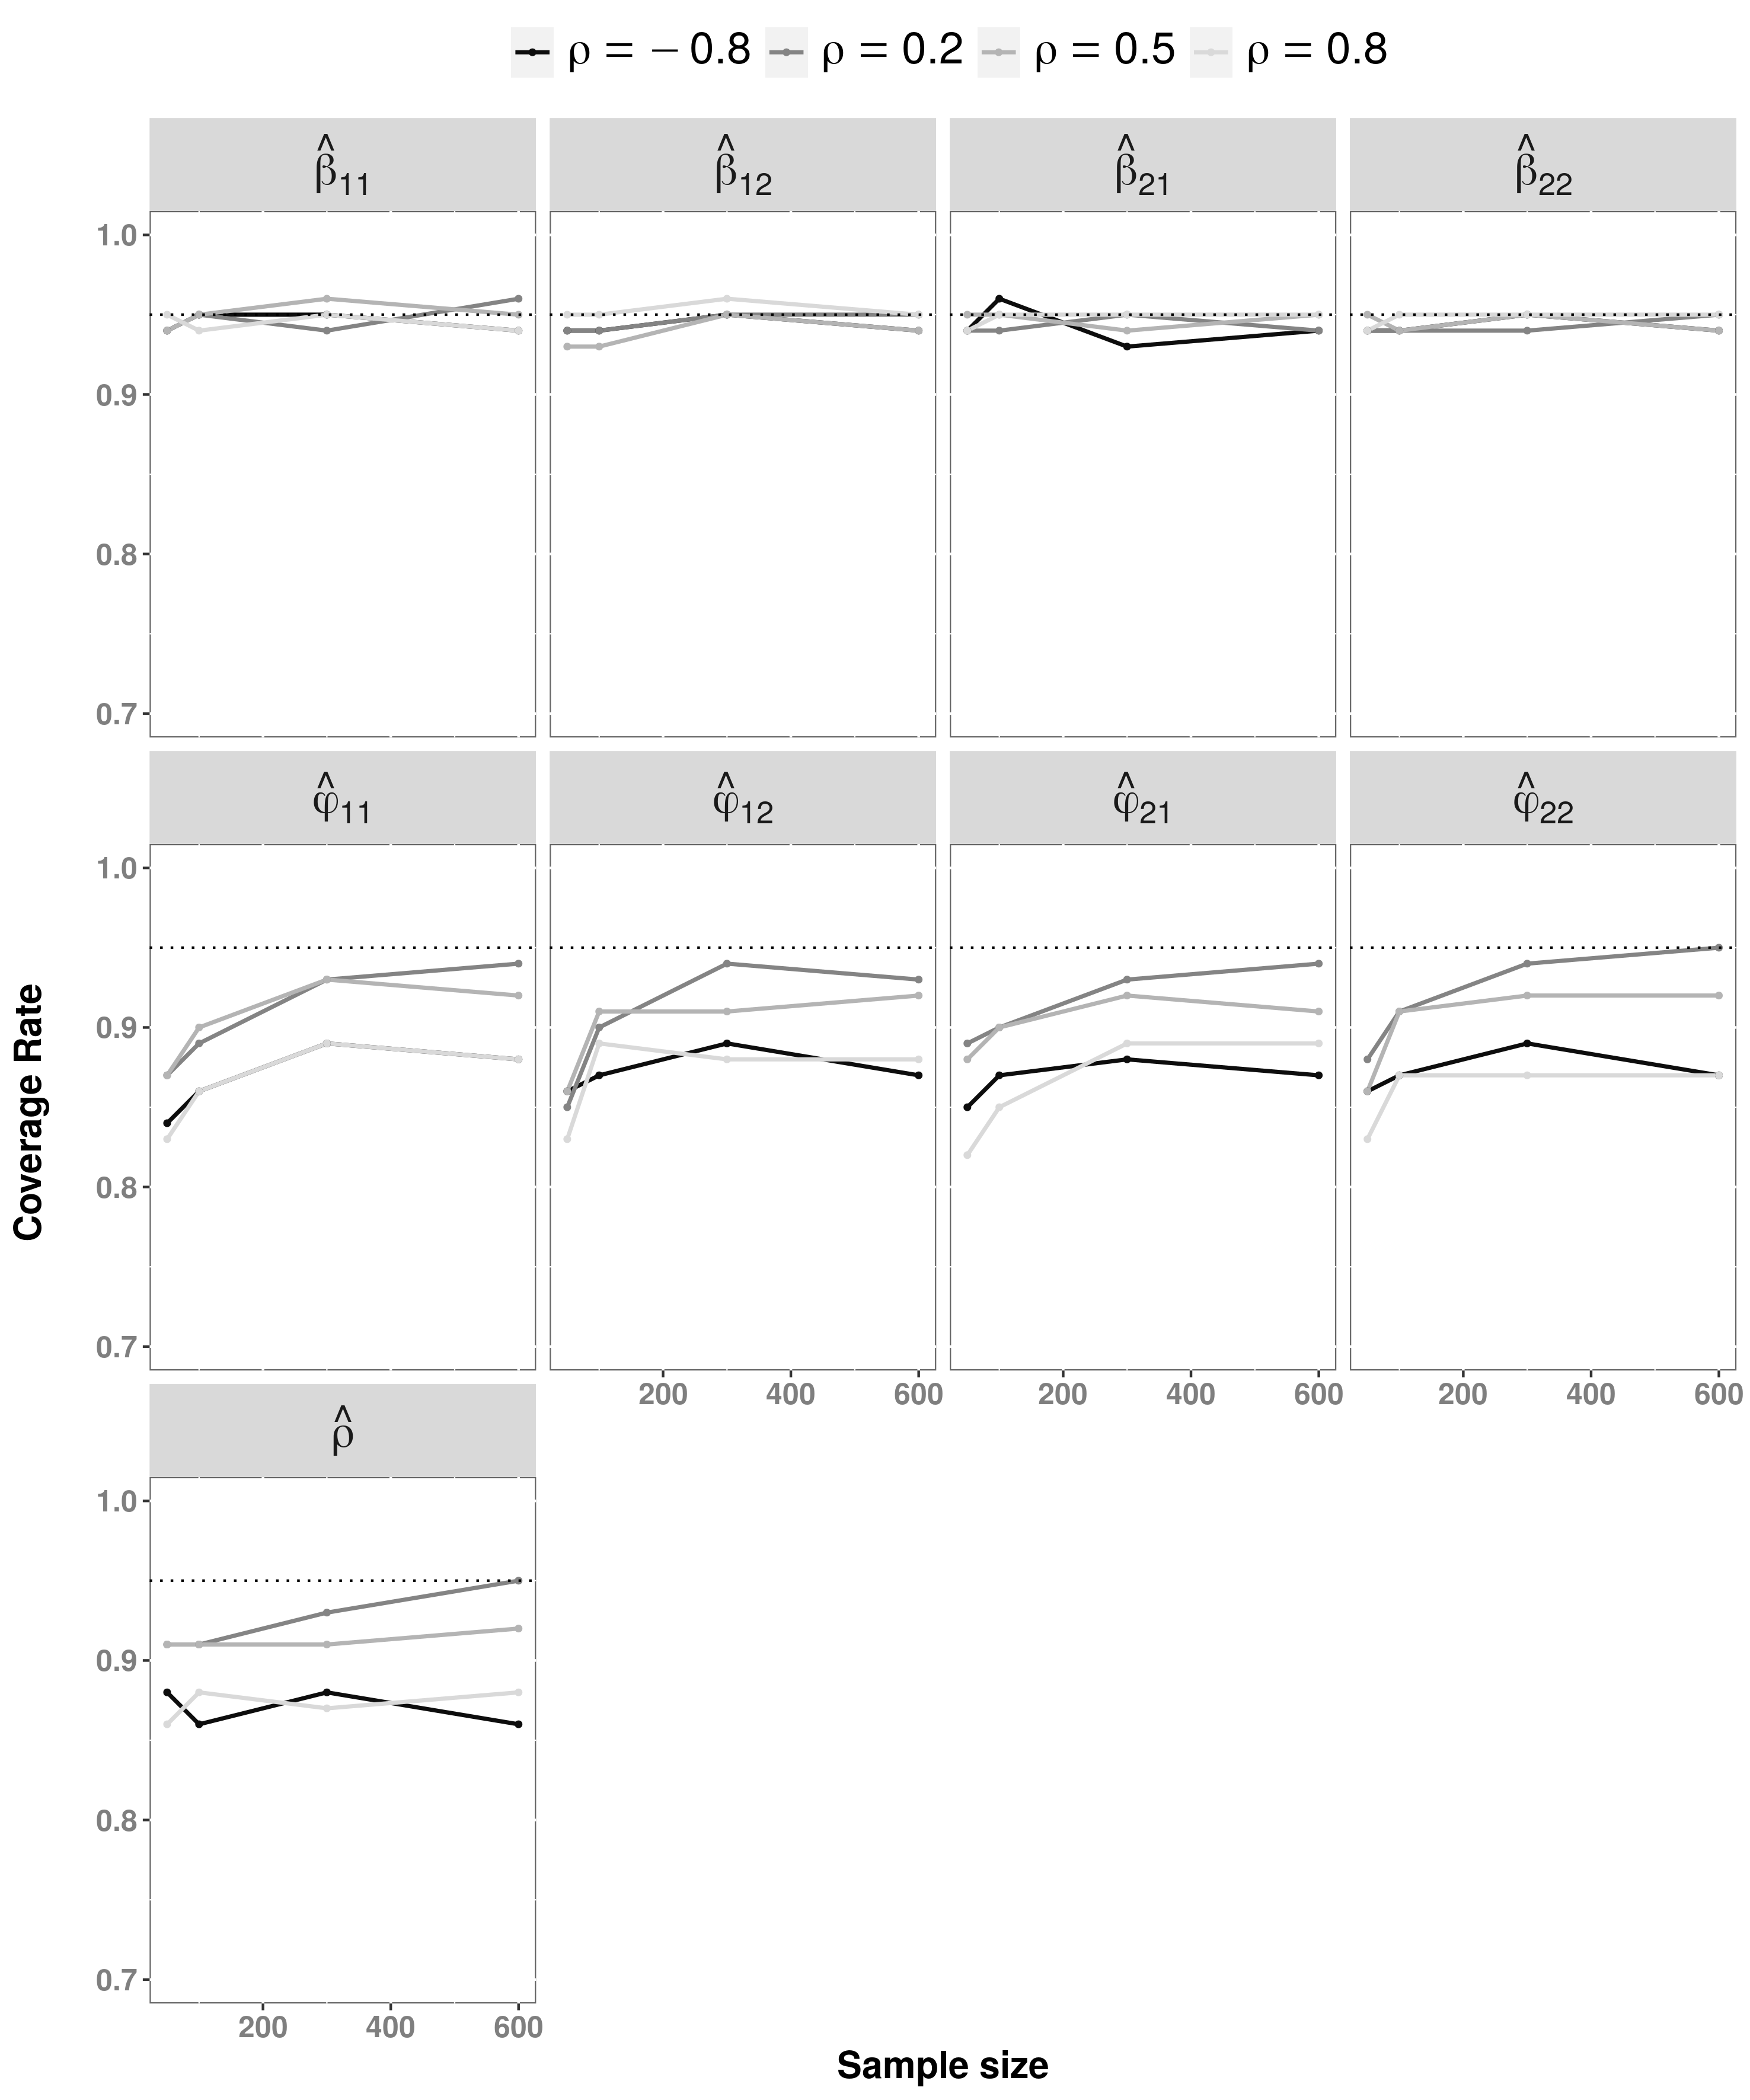
\includegraphics[width=1\textwidth]{Figure_3}
\caption{Coverage rate based on normal approximation confidence intervals with a nominal rate of $95\%$ for different sample sizes (50, 100, 300, and 600)  and correlation coefficients $\rho\in\{-0.8, 0.2, 0.5, 0.8\}$.}
\label{fig1.4}
\end{figure}

\subsection{Bootstrap approach}
To verify the coverage rate considering bootstrap confidence intervals, a parametric bootstrap simulation was performed, considering 1,000 bootstrap samples and 100 simulations, following the same previous scenarios with a sample size equal to 50 and correlation coefficients equal to $-0.8$ and $0.8$. These simulations showed some asymmetry and bias, mainly
for the dispersion and correlation coefficients, therefore bias-corrected percentile confidence intervals (BCP) were considered. ~\cite{efron1982jackknife} presented this method, in which the correction relies upon transforming the distribution to one that satisfies the symmetry condition~\citep{diciccio1988review,buckland1984monte}. Using this method, the
empirical coverage rates increased, becoming very close to the 95\% nominal coverage rate (Table \ref{table5.4}).


\begin{table}[htb]
\caption{Coverage rate based on bias-corrected percentile confidence intervals with 1,000 bootstrap samples and 100 simulations, and a nominal rate of $95\%$, for a sample size of  $n=50$ and true values for the parameters as described in Section \ref{Simulation}.}
\label{table5.4}
\begin{center}
\begin{tabular}{lrr}
	\hline
	& \multicolumn{2}{c}{Coverage rate} \\
	\hline
	Parameter	& $\rho=0.8$ & $\rho=-0.8$ \\ \hline
	$\beta_{11}$ & 0.95 & 0.96\\ 
	$\beta_{12}$ &  0.95 & 0.93 \\
	
	$\beta_{21}$& 0.98 & 0.96 \\
	
	$\beta_{22}$& 0.98 & 0.92 \\
	
	$\phi_{11}$& 0.94 & 0.95 \\ 
	$\phi_{12}$&  0.92  & 0.88\\
	$\phi_{21}$&  0.93 & 0.95 \\ 
	$\phi_{22}$& 0.91 &0.89 \\
	$\rho$ & 0.95 & 0.96\\
	\hline
\end{tabular}
\end{center}
\end{table}


Table \ref{completa} shows the results of the simulation study considering two correlation coefficients, one for each treatment. The observed average bias was low, and the larger the sample size, the lower the average bias and associated standard errors. We observed that for stronger correlations, the standard error was lower, implying empirical confidence intervals with smaller coverage than the nominal rate. Further, it is clear that the scenarios that presented better coverage, mainly for larger samples, were scenarios 1 and 4.



\begin{table}[htb]
\caption{Estimator mean bias, mean squared error (MSE) and coverage rate for the proposed model under four scenarios, which varied true parameter values. Results are based on 1,000 simulations.}\hrule\vspace{0.2cm}
\small
Scenario 1:\\
\begin{minipage}[b]{0.43\textwidth}
\label{completa}
\begin{tabular}{lrrrr} 
	& &   \multicolumn{3}{c}{Bias}  \\ 
	\cmidrule{3-5}
	
	Parameter	&  True & $n=50$ & $n=100$ & $n=300$   \\ 			\midrule 
	$\beta_{11}$ &	2&0.000
	&-0.004&	0.000\\
	$\beta_{12}$ &	3&-0.002
	&	-0.001&	0.000\\
	$\beta_{21}$&10& -0.012
	&	-0.018&	-0.017\\
	$\beta_{22}$&300&0.154
	&	-0.059&	-0.024\\
	$\phi_{11}$	&0.5& -0.020
	&	-0.013&	-0.004\\
	$\phi_{12}$&2&	-0.093
	&	-0.054&	-0.021\\
	$\phi_{21}$	&1&	-0.044
	&	-0.015&	-0.003\\
	$\phi_{22}$	&10&-0.469
	&-0.080&	0.083	\\
	$\rho_1$	&0.2&-0.005
	&-0.004&-0.001	\\
	$\rho_2$&	0.5	&-0.013
	&-0.001&	0.000\\
\end{tabular}
\end{minipage}
\begin{minipage}[b]{0.28\textwidth}
\begin{tabular}{rrr} 
	& \multicolumn{1}{c}{MSE}  &\\ 
	\midrule
	$n=50$ & $n=100$ & $n=300$   \\ 	
	\midrule 
	0.050&	0.036&	0.021\\
	0.061&	0.044&	0.026\\
	0.611&	0.441&	0.257\\
	10.584&	7.669&	4.446\\
	0.133&	0.096&	0.057\\
	0.501&	0.362&	0.213\\
	0.265&	0.194&	0.114\\
	2.501&	1.844&	1.069\\
	0.179&	0.130&	0.076\\
	0.133&	0.094&	0.055\\
\end{tabular}
\end{minipage}
\begin{minipage}[b]{.1\textwidth}
\begin{tabular}{rrr} 
	& \multicolumn{1}{c}{Coverage}  &\\ 
	\hline
	$n=50$ & $n=100$ & $n=300$   \\ 	
	\hline 
	0.94&	0.94&	0.94\\
	0.94&	0.93&	0.95\\
	0.93&	0.94&	0.95\\
	0.93&	0.95&	0.96\\
	0.88&	0.90&	0.92\\
	0.87&	0.90&	0.91\\
	0.87&	0.90&	0.93\\
	0.87&	0.90&	0.91\\
	0.88&	0.92&	0.93\\
	0.88&	0.89&	0.91\\
\end{tabular}
\end{minipage}
\\\hrule\vspace{0.2cm}
Scenario 2:\\
\begin{minipage}[b]{.43\textwidth}
\begin{tabular}{lrrrr} 
	& &   \multicolumn{3}{c}{Bias}  \\ 
	\cmidrule{3-5}
	Parameter	&  True & $n=50$ & $n=100$ & $n=300$   \\ 			\midrule 
	$\beta_{11}$ &	2&-0.002&	-0.001&	0.001\\
	$\beta_{12}$ &	3&-0.002&	0.001&	0.001\\
	$\beta_{21}$&10& 0.021&	0.006&	-0.004\\
	$\beta_{22}$&300&-0.093&	0.207&	0.078\\
	$\phi_{11}$	&0.5&-0.015&	-0.014&	-0.005\\
	$\phi_{12}$&2&	-0.059&	-0.048&	-0.031\\
	$\phi_{21}$	&1&	-0.036&	-0.021&	-0.012\\
	$\phi_{22}$	&10&-0.283&	-0.281&	-0.130\\
	$\rho_1$	&0.2&-0.011&	0.003&	0.000\\
	$\rho_2$&	0.8	&-0.006&	-0.002&	-0.002\\
\end{tabular}
\end{minipage}
\begin{minipage}[b]{.28\textwidth}
\begin{tabular}{rrr} 
	& \multicolumn{1}{c}{MSE} & \\ 
	\hline
	$n=50$ & $n=100$ & $n=300$   \\ 	
	\midrule 
	0.051&	0.036&	0.021\\
	0.062&	0.044&	0.026\\
	0.614&	0.440&	0.256\\
	10.682&	7.599&	4.435\\
	0.134&	0.096&	0.057\\
	0.450&	0.321&	0.187\\
	0.267&	0.193&	0.113\\
	2.252&	1.597&	0.939\\
	0.180&	0.129&	0.076\\
	0.058&	0.040&	0.023\\
\end{tabular}
\end{minipage}
\begin{minipage}[b]{.1\textwidth}
\begin{tabular}{rrr} 
	& \multicolumn{1}{c}{Coverage} & \\ 
	\hline
	n=50 & n=100 & n=300   \\ 	
	\midrule 
	0.91&	0.95&	0.94\\
	0.92&	0.94&	0.94\\
	0.94&	0.94&	0.94\\
	0.92&	0.94&	0.95\\
	0.89&	0.89&	0.93\\
	0.86&	0.87&	0.87\\
	0.89&	0.91&	0.93\\
	0.86&	0.86&	0.88\\
	0.90&	0.91&	0.95\\
	0.83&	0.86&	0.87\\ 		
\end{tabular}
\end{minipage}
\\\hrule\vspace{0.2cm}
Scenario 3:\\
\begin{minipage}[b]{.43\textwidth}	
\begin{tabular}{lrrrr} 
	& &   \multicolumn{3}{c}{Bias}  \\ 
	\cmidrule{3-5}
	Parameter	&  True & $n=50$ & $n=100$ & $n=300$   \\ 			\midrule 
	$\beta_{11}$ &	2&-0.001&	0.000&	0.000\\
	$\beta_{12}$ &	3&0.001&	0.001&	0.001\\
	$\beta_{21}$&10&-0.013&	-0.025&	-0.007\\
	$\beta_{22}$&300&-0.149&	-0.321&	0.245\\
	$\phi_{11}$	&0.5& -0.014&	-0.014&	-0.001\\
	$\phi_{12}$&2&	-0.109&	-0.050&	-0.029\\
	$\phi_{21}$	&1&	-0.030&	-0.010&	-0.002\\
	$\phi_{22}$	&10&-0.239&	-0.268&	-0.100\\
	$\rho_1$ &-0.8	&0.005&	0.007&	0.002\\
	$\rho_2$&	0.2	&
	0.004&	-0.003&	-0.004\\
\end{tabular}
\end{minipage}
\begin{minipage}[b]{.28\textwidth} 		
\begin{tabular}{rrr} 
	& \multicolumn{1}{c}{MSE}  &\\ 
	\hline
	$n=50$ & $n=100$ & $n=300$   \\ 	
	\hline 
	0.051&	0.036&	0.021\\
	0.061&	0.044&	0.026\\
	0.615&	0.442&	0.257\\
	10.699&	7.599&	4.444\\
	0.112&	0.080&	0.047\\
	0.524&	0.384&	0.225\\
	0.225&	0.163&	0.095\\
	2.701&	1.918&	1.130\\
	0.057&	0.041&	0.023\\
	0.178&	0.130&	0.076\\ 	
\end{tabular}
\end{minipage}
\begin{minipage}[b]{.1\textwidth} 		
\begin{tabular}{rrr} 
	& \multicolumn{1}{c}{Coverage} &  \\ 
\hline
	$n=50$ & $n=100$ & $n=300$   \\ 	
	\midrule 
	0.94&	0.93&	0.93\\
	0.92&	0.94&	0.95\\
	0.92&	0.93&	0.95\\
	0.94&	0.93&	0.94\\
	0.83&	0.85&	0.89\\
	0.86&	0.91&	0.93\\
	0.84&	0.86&	0.89\\
	0.88&	0.91&	0.94\\
	0.85&	0.84&	0.85\\
	0.88&	0.93&	0.94\\	
\end{tabular}
\end{minipage}
\\\hrule\vspace{0.2cm}
Scenario 4:\\
\begin{minipage}[b]{.43\textwidth}
\begin{tabular}{lrrrr} 
	& &   \multicolumn{3}{c}{Bias}  \\ 
	\cmidrule{3-5}
	Parameter	&  True & $n=50$ & $n=100$ & $n=300$   \\ 			\midrule 
	$\beta_{11}$ &	2&-0.003&	0.001&	-0.001\\
	$\beta_{12}$ &	3&-0.001&	0.002&	0.001\\
	$\beta_{21}$&10& -0.041&	-0.013&	-0.002\\
	$\beta_{22}$&300&-0.137&	-0.179&	0.361\\
	$\phi_{11}$	&0.5&-0.017&	-0.010&	-0.004\\
	$\phi_{12}$&2&-0.085&	-0.062&	-0.035\\
	$\phi_{21}$	&1&-0.035&	-0.014&	-0.009\\
	$\phi_{22}$	&10&-0.448&	-0.264&	-0.071\\
	$\rho_1$	&-0.2&0.004&	0.000&	0.002\\
	$\rho_2$&	0.5	&-0.015&	-0.008&	-0.005\\
	%\hline
\end{tabular}
\end{minipage}
\begin{minipage}[b]{.28\textwidth}
\begin{tabular}{rrr} 
	& \multicolumn{1}{c}{MSE}  &\\
	\hline
	$n=50$ & $n=100$ & $n=300$   \\ 	
	\midrule 
	0.051&	0.036&	0.021\\
	0.061&	0.044&	0.025\\
	0.612&	0.441&	0.256\\
	10.583&	7.597&	4.450\\
	0.134&	0.097&	0.057\\
	0.503&	0.361&	0.212\\
	0.267&	0.194&	0.113\\
	2.506&	1.815&	1.072\\
	0.179&	0.130&	0.076\\
	0.134&	0.095&	0.055\\	
	%\hline
\end{tabular}
\end{minipage}
\begin{minipage}[b]{.1\textwidth}	
\begin{tabular}{rrr} 
	& \multicolumn{1}{c}{Coverage} &  \\ 
	\hline
	$n=50$ & $n=100$ & $n=300$   \\ 	
	\hline 
	0.94&	0.94&	0.94\\
	0.94&	0.94&	0.95\\
	0.93&	0.96&	0.94\\
	0.94&	0.95&	0.95\\
	0.88&	0.91&	0.92\\
	0.88&	0.90&	0.91\\
	0.88&	0.92&	0.91\\
	0.86&	0.88&	0.91\\
	0.88&	0.94&	0.93\\
	0.88&	0.90&	0.90\\	
	%\hline
\end{tabular}
\end{minipage}
\hrule
\end{table}












\section{Discussion}
\label{s:discuss}

In this work, we proposed a bivariate framework to jointly model count and continuous responses. Our approach represents an attractive and flexible framework for studying two variables jointly and is widely applicable. This alternative considered a bivariate normal distribution, modelling the variance-covariance matrix so that the characteristics of the data, such as over- or underdispersion for count data, and heterogeneity of variances for continuous data can be modelled. As expected, the normal approximation performed better with larger sample sizes. The advantage of this methodology is that it is possible to incorporate correlation, to jointly model the variable responses and to assume an associated probability distribution. One drawback of our approach is that issues may arise for small sample sizes, including biased dispersion estimates and a true coverage rate of the confidence intervals for the parameters smaller than the nominal rate. So it is necessary to carefully analyse very small samples, doing descriptive analyses before fitting the model, and checking if the obtained results have a practical interpretation.

We observed in the simulation studies that even for large samples, when $\rho = -0.8$ and $\rho = 0.8$,  the coverage rate of the correlation parameters is close to $90\%$ instead of $95\%$. This is possibly because the true correlation value is close to the boundary of the parametric space. When  $\rho \approx 1$,  the range limits are automatically limited by 1 or $-1$, then the variation of the parameter space is smaller. This became more evident by observing Figure \ref{fig1.3}, which showed that the standard errors for the correlation coefficients are lower for higher correlations. This is not reflected in the regression coefficients, due to the fact that $\boldsymbol{\hat\beta}$ varies very little for different values of $\phi$ and $\rho$. However, the coverage rate for the dispersion parameters also depends on the correlation parameter value, and the higher the correlation, the lower the coverage rate.  These problems are expected when it comes to estimates at the limit of the parametric space, especially with smaller samples. Despite these limitations, we concluded that the model generally behaves as expected, with unbiased, consistent, and accurate estimates.


Several extensions to the proposed bivariate model are possible (and currently in progress). These extensions include modelling correlation between observations taken on the same experimental unit, e.g., longitudinal data or repeated measurements. In this case, the variance-covariance matrix needs to be extended, allowing to incorporate the dependent measures taken on the same subject.  This extension will be carried out by generalising $\boldsymbol{\Sigma} = \mathbf{D_\phi D_\mu} + \mathbf{ZGZ'}$, where $\mathbf{Z}$ is the matrix of known grouping factors reflecting correlated observations or how the response evolves overtime for each subject and $\mathbf{G}$ a general variance-covariance matrix. However, it is also necessary to include a link function for the dispersion parameter, so that it does not yield a negative maximum likelihood estimate.
%  Here, we create the bibliographic entries manually, following the
%  journal style.  If you use this method or use natbib, PLEASE PAY
%  CAREFUL ATTENTION TO THE BIBLIOGRAPHIC STYLE IN A RECENT ISSUE OF
%  THE JOURNAL AND FOLLOW IT!  Failure to follow stylistic conventions
%  just lengthens the time spend copyediting your paper and hence its
%  position in the publication queue should it be accepted.

%  We greatly prefer that you incorporate the references for your
%  article into the body of the article as we have done here 
%  (you can use natbib or not as you choose) than use BiBTeX,
%  so that your article is self-contained in one file.
%  If you do use BiBTeX, please use the .bst file that comes with 
%  the distribution.  In this case, replace the thebibliography
%  environment below by 
%
\bibliographystyle{biom} \bibliography{Cap2}



%  If your paper refers to supporting web material, then you MUST
%  include this section!!  See Instructions for Authors at the journal
%  website http://www.biometrics.tibs.org



%\section*{Supporting Information}

%Web ix A, referenced in Section~\ref{s:model}, is available with
%this paper at the Biometrics website on Wiley Online
%Library.\vspace*{-8pt}

\appendix


	 \renewcommand{\theequation}{A.\arabic{equation}}
	% redefine the command that creates the equation no.
	\setcounter{equation}{0}  % reset counter 
	
\section*{Appendix A: Estimation and Inference for Section 3}

Taking one of the response outcomes $\mathbf {Y} _i $, from here we will omit the index $ i $ to improve readability. Asymptotically  $\boldsymbol{Y} \sim N({\boldsymbol{\mu}},\boldsymbol{\Sigma}= \mathbf{D_\phi}\mathbf{D_\mu})$, we can write the log-likelihood as
\begin{equation}\label{eq12}
\begin{array}{l}
\log \mathcal{L}(\boldsymbol{\mu},\boldsymbol{\Sigma}| \mathbf{y})= l(\boldsymbol{\mu},\boldsymbol{\Sigma}| \mathbf{y})= -\frac{1}{2}\{\log |\boldsymbol{\Sigma}| +  (\mathbf{y}-\boldsymbol{\mu})'\boldsymbol{\Sigma}^{-1} (\mathbf{y}-\boldsymbol{\mu})\} + \mbox{const.}



%= -\frac{1}{2}\log |\mathbf{D_\phi}\mathbf{D_\mu}| - \frac{1}{2} (\mathbf{y}-\boldsymbol{\mu})'(\mathbf{D_\phi}\mathbf{D_\mu})^{-1} (\mathbf{y}-\boldsymbol{\mu})\\~\\

%  =	\{- \frac{1}{2}\log|\mathbf{D_\phi}|-  \frac{1}{2} \log|\mathbf{D_\mu}|  - \frac{1}{2} (\mathbf{y}-\boldsymbol{\mu})'(\mathbf{D_\phi}\mathbf{D_\mu})^{-1} (\mathbf{y}-\boldsymbol{\mu}) \}

\end{array}
\end{equation}

Differentiating with respect to $\boldsymbol{\Sigma}$ is straightforward:
\begin{equation}
\begin{array}{l}
\dfrac{\partial l}{\partial \boldsymbol{\Sigma}} =\dfrac{\partial l}{\partial \boldsymbol{\Sigma}} \{-\frac{1}{2}\log |\boldsymbol{\Sigma}| - \frac{1}{2} (\mathbf{y}-\boldsymbol{\mu})'\boldsymbol{\Sigma}^{-1} (\mathbf{y}-\boldsymbol{\mu})\}



%= -\frac{1}{2}\log |\mathbf{D_\phi}\mathbf{D_\mu}| - \frac{1}{2} (\mathbf{y}-\boldsymbol{\mu})'(\mathbf{D_\phi}\mathbf{D_\mu})^{-1} (\mathbf{y}-\boldsymbol{\mu})\\~\\

%  =	\{- \frac{1}{2}\log|\mathbf{D_\phi}|-  \frac{1}{2} \log|\mathbf{D_\mu}|  - \frac{1}{2} (\mathbf{y}-\boldsymbol{\mu})'(\mathbf{D_\phi}\mathbf{D_\mu})^{-1} (\mathbf{y}-\boldsymbol{\mu}) \}
\end{array}
\end{equation}\\
as $\dfrac{\partial}{\partial A} \log|A| = A' \quad \mbox{and} \quad \dfrac{\partial \mathbf{a' X^{-1} b}}{\partial \mathbf{X}}  = -(\mathbf{X}^{-1})' \mathbf{(ab)' (X^{-1})'}$. Then, 

\begin{equation}
\begin{array}{l}
\dfrac{\partial l}{\partial \boldsymbol{\Sigma}} = -\frac{1}{2}(\boldsymbol{\Sigma}^{-1})'+\frac{1}{2}(\boldsymbol{\Sigma}^{-1})'(\mathbf{y}-\boldsymbol{\mu})(\mathbf{y}-\boldsymbol{\mu})'(\boldsymbol{\Sigma}^{-1})'

\end{array}
\end{equation}
and
\begin{equation*}
\begin{array}{l}
\dfrac{\partial l}{\partial \boldsymbol{\Sigma}} \dfrac{\partial \boldsymbol{\Sigma}}{\partial \mathbf{D_\phi}}= \left[-\frac{1}{2}(\boldsymbol{\Sigma}^{-1})'+\frac{1}{2}(\boldsymbol{\Sigma}^{-1})'(\mathbf{y}-\boldsymbol{\mu})(\mathbf{y}-\boldsymbol{\mu})'(\boldsymbol{\Sigma}^{-1})'\right] \circ \mathbf{D_\mu}\\~\\

= \left[-\frac{1}{2}(\mathbf{(D_\phi D_\mu)}^{-1})'+\frac{1}{2}(\mathbf{(D_\phi D_\mu)}^{-1})'(\mathbf{y}-\boldsymbol{\mu})(\mathbf{y}-\boldsymbol{\mu})'(\mathbf{(D_\phi D_\mu)}^{-1})'\right] \circ \mathbf{D_\mu}\\~\\

= -\frac{1}{2}(\mathbf{(D_\phi D_\mu)}^{-1})'\circ\mathbf{D_\mu}+\frac{1}{2}(\mathbf{(D_\phi D_\mu)}^{-1})'(\mathbf{y}-\boldsymbol{\mu})(\mathbf{y}-\boldsymbol{\mu})'(\mathbf{(D_\phi D_\mu)}^{-1})'\circ\mathbf{D_\mu} \\~\\

= -\frac{1}{2}(\mathbf{ D_\phi^{-1})'(D_\mu^{-1})'}\circ\mathbf{D_\mu}+\frac{1}{2}(\mathbf{ D_\phi^{-1})'(D_\mu^{-1})'}(\mathbf{y}-\boldsymbol{\mu})(\mathbf{y}-\boldsymbol{\mu})'(\mathbf{ D_\phi^{-1})'(D_\mu^{-1})'}\circ\mathbf{D_\mu} \\~\\

= -\frac{1}{2}\mathbf{ (D_\phi^{-1})'}+\frac{1}{2}(\mathbf{ D_\phi^{-1})(D_\mu^{-1}})'(\mathbf{y}-\boldsymbol{\mu})(\mathbf{y}-\boldsymbol{\mu})'(\mathbf{D_\phi^{-1})'}.

\end{array}
\end{equation*}
where $\mathbb{I}$ is an $n \times n$ identity matrix and $\circ$ the Hadamard product. If \textbf{A} is diagonal, then $\textbf{A'} = \textbf{A}$ and

\begin{equation*}
\begin{array}{l}
\dfrac{\partial l}{\partial \boldsymbol{\Sigma}} \dfrac{\partial \boldsymbol{\Sigma}}{\partial \mathbf{D_\phi}}\dfrac{\partial \mathbf{D_\phi}}{\partial \boldsymbol{\phi}}=[-\frac{1}{2}\mathbf{ D_\phi^{-1}}+\frac{1}{2}\mathbf{ D_\phi^{-1}D_\mu^{-1}}(\mathbf{y}-\boldsymbol{\mu})(\mathbf{y}-\boldsymbol{\mu})'\mathbf{ D_\phi^{-1}}]\circ \mathbb{I}\\~\\     
\end{array}
\end{equation*}
\begin{equation}\label{eq3}
= -\frac{1}{2}\mbox{diag}\mathbf{ (X_\phi \boldsymbol{\phi})^{-1}}\circ \mathbb{I}+\frac{1}{2}\mbox{diag}\mathbf{ (X_\phi \boldsymbol{\phi})^{-1}D_\mu^{-1}}(\mathbf{y}-\boldsymbol{\mu})(\mathbf{y}-\boldsymbol{\mu})'\mbox{diag}\mathbf{( X_\phi \boldsymbol{\phi})^{-1}}\circ \mathbb{I}.
\end{equation}\\
Equating (\ref{eq3}) to zero yields

\begin{equation}\label{eqphi}
\begin{array}{l}
-\frac{1}{2}\mbox{diag}\boldsymbol{ (\mathbf{X}_\phi \hat{\phi})^{-1}}\circ \mathbb{I}+\frac{1}{2}\mbox{diag}\boldsymbol{ (X_\phi \hat{\phi})^{-1}\mathbf{D}_\mu^{-1}}(\mathbf{y}-\boldsymbol{\mu})(\mathbf{y}-\boldsymbol{\mu})'\mbox{diag}\boldsymbol{( \mathbf{X}_\phi \hat{\phi})^{-1}}\circ \mathbb{I} =0 \nonumber\\~\\

\Rightarrow \mbox{diag}\boldsymbol{ (X_\phi \hat{\phi})^{-1}}\circ \mathbb{I}=\mbox{diag}\boldsymbol{ (\mathbf{X}_\phi \hat{\phi})^{-1}\mathbf{D}_\mu^{-1}}(\mathbf{y}-\boldsymbol{\mu})(\mathbf{y}-\boldsymbol{\mu})'\mbox{diag}\boldsymbol{( \mathbf{X}_\phi \hat{\phi})^{-1}} \nonumber\circ \mathbb{I}\\~\\

%\mbox{diag}\boldsymbol{ (\mathbf{X}_\phi \hat{\phi})}\mbox{diag}\boldsymbol{ (\mathbf{X}_\phi \hat{\phi})^{-1}}\mbox{diag}\boldsymbol{ (\mathbf{X}_\phi \hat{\phi})}=\mbox{diag}\boldsymbol{ (\mathbf{X}_\phi \hat{\phi})}\mbox{diag}\boldsymbol{ (\mathbf{X}_\phi \hat{\phi})^{-1}\mathbf{D}_\mu^{-1}}(\mathbf{y}-\boldsymbol{\mu})(\mathbf{y}-\boldsymbol{\mu})'\circ \mathbb{I}\\\hspace{13cm}\mbox{diag}\boldsymbol{( \mathbf{X}_\phi \hat{\phi})^{-1}}\mbox{diag}\boldsymbol{ (\mathbf{X}_\phi \hat{\phi})}\nonumber \\~\\


\Rightarrow\mbox{diag}\boldsymbol{ (\mathbf{X}_\phi \hat{\phi})}=\mathbf{D_\mu^{-1}}(\mathbf{y}-\boldsymbol{\mu})(\mathbf{y}-\boldsymbol{\mu})'\circ \mathbb{I}\nonumber.\\

\end{array}
\end{equation}\\
Post-multiplying both sides by $\mathbb{J}_{n \times 1}$, where $\mathbb{J}$ is an $n \times 1$ vector of 1s yields
\begin{equation}
 \boldsymbol{\mathbf{X}_\phi \hat{\phi}} = \mathbf{(D_\mu^{-1}}(\mathbf{y}-\boldsymbol{\mu})(\mathbf{y}-\boldsymbol{\mu})'\circ \mathbb{I}) \mathbb{J}
\end{equation}
Finally, pre-multiplying both sides by $\mathbf{(X_\phi'X_\phi)^{-1}X_\phi'}$ yields
\begin{equation}
\boldsymbol{\hat{\phi}} = \mathbf{(X_\phi'X_\phi)^{-1}X_\phi'}\mathbf{\{(D_\mu^{-1}}(\mathbf{y}-\boldsymbol{\mu})(\mathbf{y}-\boldsymbol{\mu})'\circ \mathbb{I}) \mathbb{J}\} 
\end{equation}

%\captionsetup{labelformat=AppendixTables}
%\setcounter{table}{0}

%We presented all simulation studies carried out with the proposed model. We investigated
%model performance for two values of $\rho$ under 14 different scenarios, varying sample
%size, from 1000 simulations. We obtained the bias, the  mean square error (MSE) and the coverage rate(see Table 5).



\end{document}